\documentclass[a4paper,12pt,twoside,openany]{report}
%
% Wzorzec pracy dyplomowej
% J. Starzynski (jstar@iem.pw.edu.pl) na podstawie pracy dyplomowej
% mgr. inż. Błażeja Wincenciaka
% Wersja 0.1 - 8 października 2016
%
\usepackage{polski}
\usepackage{helvet}
\usepackage{xunicode}
\usepackage{fontspec}
\defaultfontfeatures{Mapping=tex-text}
\usepackage{anyfontsize}
\usepackage{xltxtra}
\usepackage{graphicx}
\usepackage{tabularx}
\usepackage{array}
\usepackage[polish]{babel}
\usepackage{subfigure}
\usepackage{amsfonts}
\usepackage{verbatim}
\usepackage{indentfirst}
\usepackage[xetex]{hyperref}
\usepackage[style=numeric]{biblatex}
\usepackage{placeins}
\usepackage{xcolor}
\usepackage{mdframed}
\usepackage{float}

\maxdeadcycles=900000000


% rozmaite polecenia pomocnicze
% gdzie rysunki?
\newcommand{\ImgPath}{./img}

% oznaczenie rzeczy do zrobienia/poprawienia
\newcommand{\TODO}{\textbf{TODO}}


% wyroznienie slow kluczowych
\newcommand{\tech}{\texttt}

\newcommand{\omnetpp}{OMNeT++}

% na oprawe (1.0cm - 0.7cm)*2 = 0.6cm
% na oprawe (1.1cm - 0.7cm)*2 = 0.8cm
%  oddsidemargin lewy margines na nieparzystych stronach
% evensidemargin lewy margines na parzystych stronach
\def\oprawa{1.05cm}
\addtolength{\oddsidemargin}{\oprawa}
\addtolength{\evensidemargin}{-\oprawa}

% table span multirows
\usepackage{multirow}
\usepackage{enumitem}	% enumitem.pdf
\setlist{listparindent=\parindent, parsep=\parskip} % potrzebuje enumitem

%%%%%%%%%%%%%%% Dodatkowe Pakiety %%%%%%%%%%%%%%%%%
\usepackage{prmag2017}   % definiuje komendy opieku,nrindeksu, rodzaj pracy, ...

\begin{document}

\begin{figure}[H]
	\begin{center}
		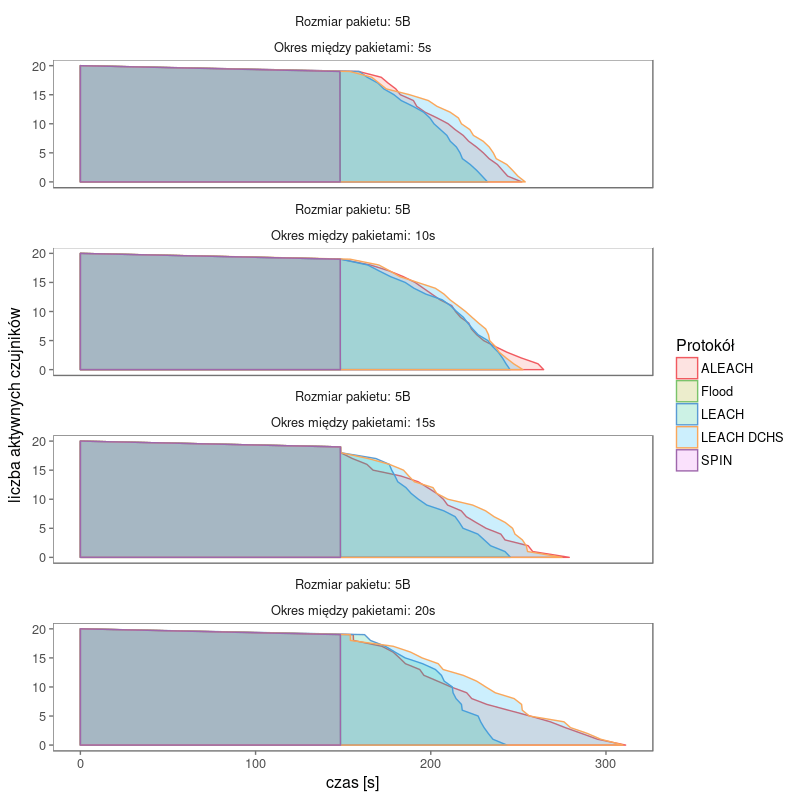
\includegraphics[scale=0.7]{\ImgPath/charts/alive_nodes_normal_20sensors_row1.png}
	\end{center}
	\caption{Aktywne węzły - 20 czujników, rozkład normalny, rozmiar pakietu: 5B}
\end{figure}

\begin{figure}[H]
	\begin{center}
		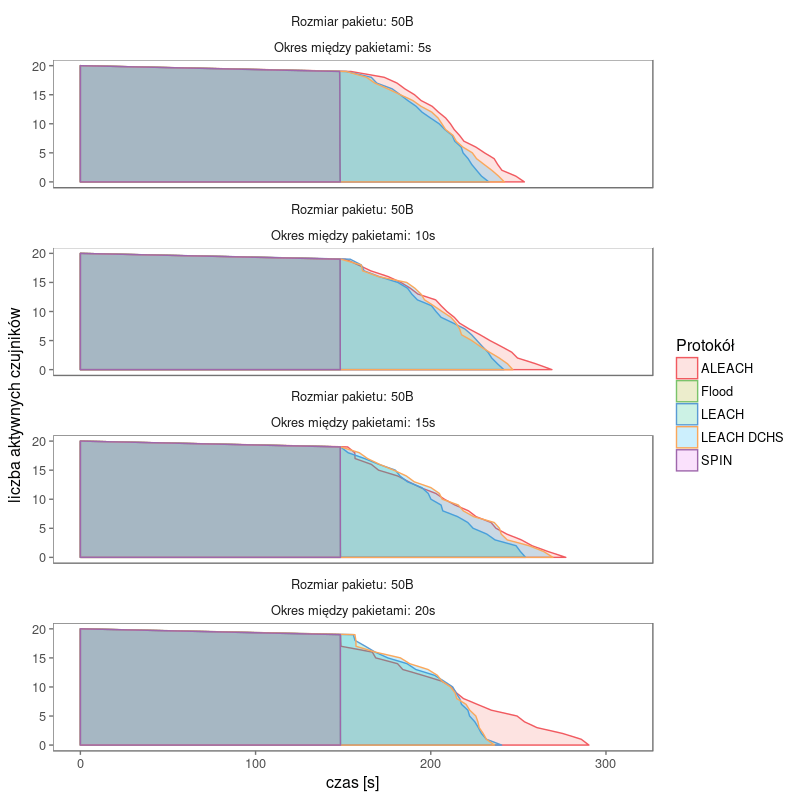
\includegraphics[scale=0.7]{\ImgPath/charts/alive_nodes_normal_20sensors_row2.png}
	\end{center}
	\caption{Aktywne węzły - 20 czujników, rozkład normalny, rozmiar pakietu: 50B}
\end{figure}

\begin{figure}[H]
	\begin{center}
		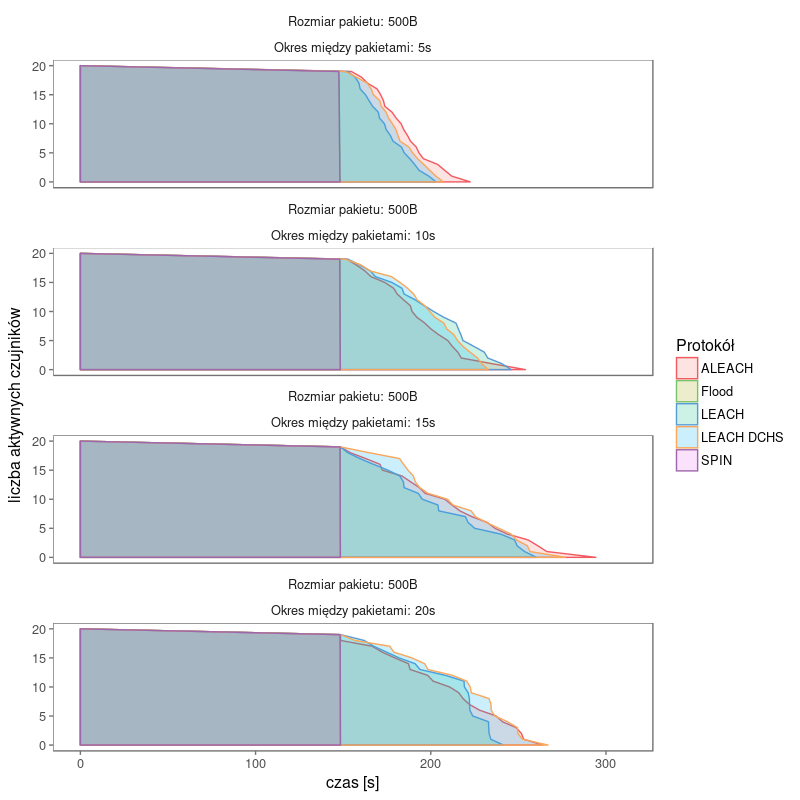
\includegraphics[scale=0.7]{\ImgPath/charts/alive_nodes_normal_20sensors_row3.png}
	\end{center}
	\caption{Aktywne węzły - 20 czujników, rozkład normalny, rozmiar pakietu: 500B}
\end{figure}

Przy rozmiarze pakietu 5000B jedynym przypadkiem w, którym ALEACH działa gorzej jest okres pomiędzy pakietami wynoszący 10s.

\begin{figure}[H]
	\begin{center}
		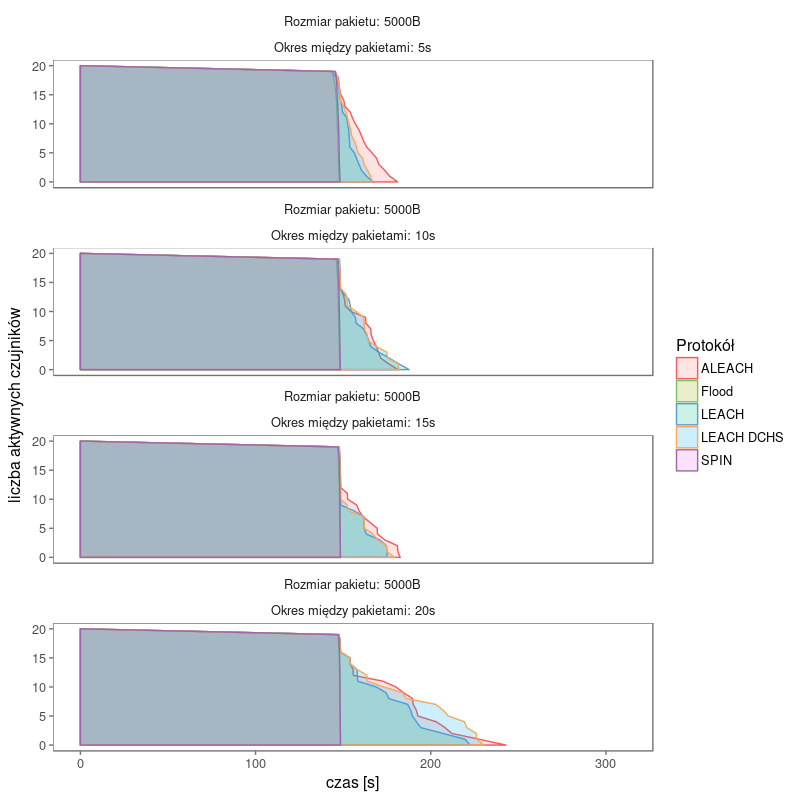
\includegraphics[scale=0.7]{\ImgPath/charts/alive_nodes_normal_20sensors_row4.png}
	\end{center}
	\caption{Aktywne węzły - 20 czujników, rozkład normalny, rozmiar pakietu: 5000B}
\end{figure}

\begin{figure}[H]
	\begin{center}
		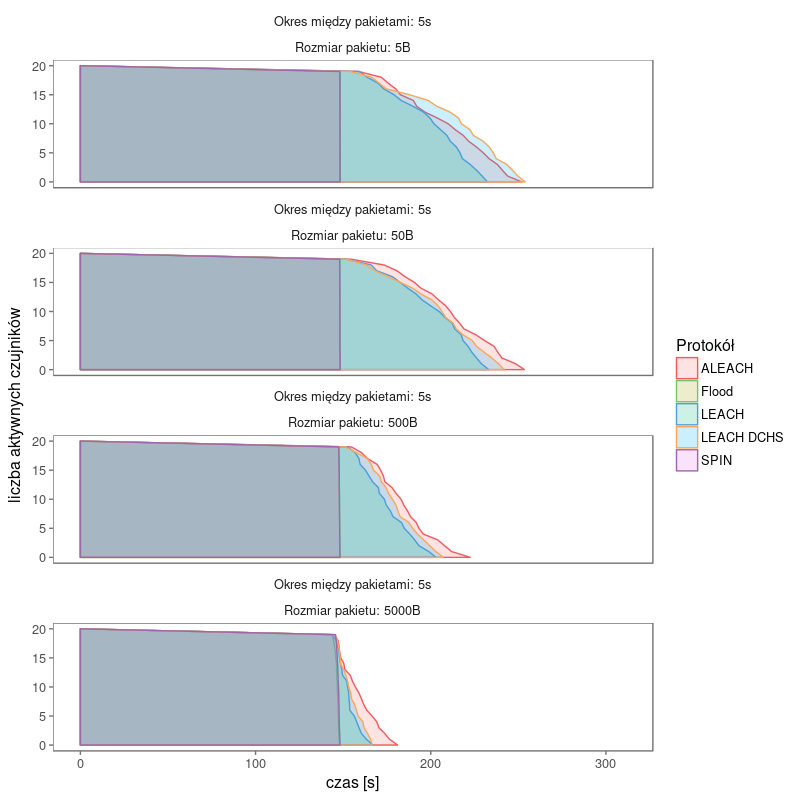
\includegraphics[scale=0.7]{\ImgPath/charts/alive_nodes_normal_20sensors_col1.png}
	\end{center}
	\caption{Aktywne węzły - 20 czujników, rozkład normalny, okres pomiędzy pakietami: 5s}
\end{figure}

\begin{figure}[H]
	\begin{center}
		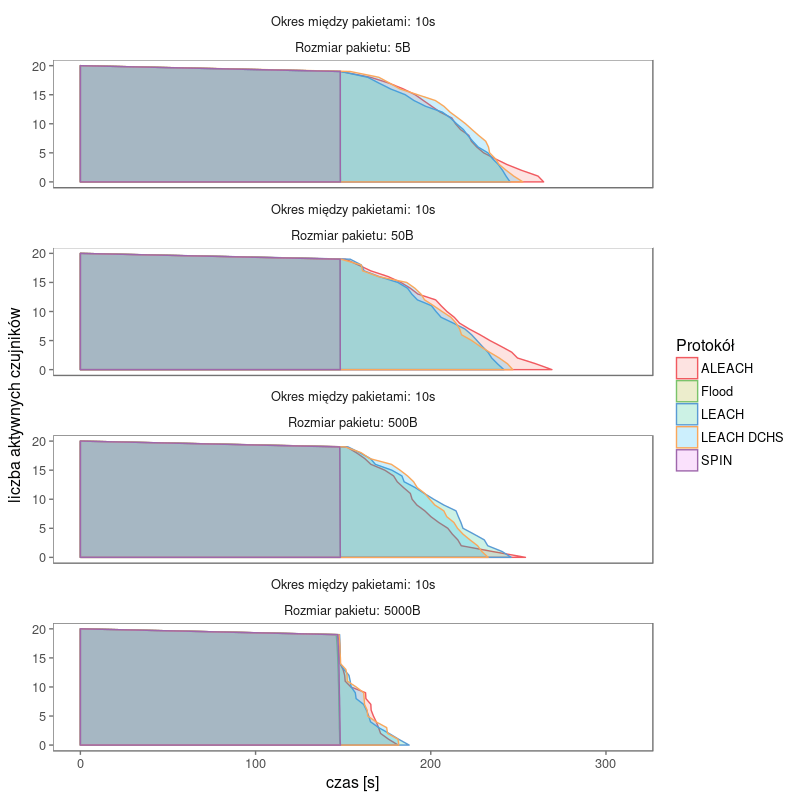
\includegraphics[scale=0.7]{\ImgPath/charts/alive_nodes_normal_20sensors_col2.png}
	\end{center}
	\caption{Aktywne węzły - 20 czujników, rozkład normalny, okres pomiędzy pakietami: 10s}
\end{figure}

\begin{figure}[H]
	\begin{center}
		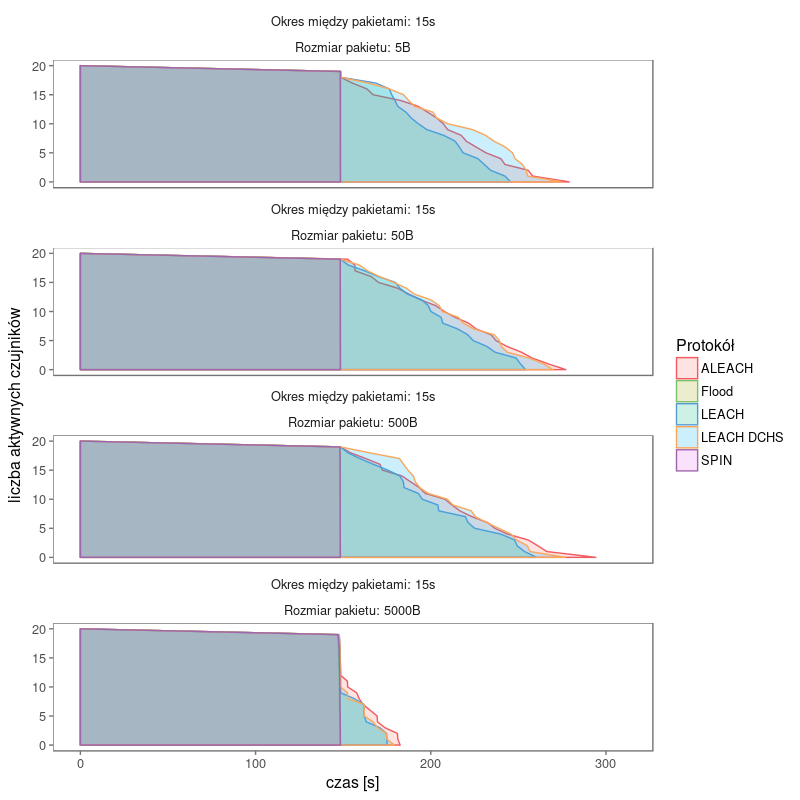
\includegraphics[scale=0.7]{\ImgPath/charts/alive_nodes_normal_20sensors_col3.png}
	\end{center}
	\caption{Aktywne węzły - 20 czujników, rozkład normalny, okres pomiędzy pakietami: 15s}
\end{figure}

\begin{figure}[H]
	\begin{center}
		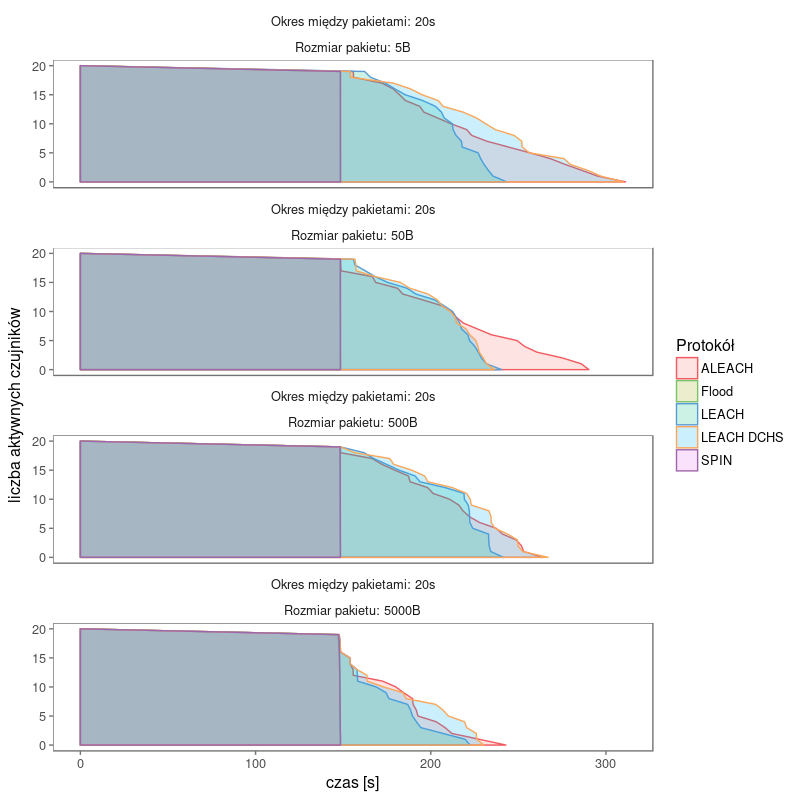
\includegraphics[scale=0.7]{\ImgPath/charts/alive_nodes_normal_20sensors_col4.png}
	\end{center}
	\caption{Aktywne węzły - 20 czujników, rozkład normalny, okres pomiędzy pakietami: 20s}
\end{figure}

\begin{figure}[H]
	\begin{center}
		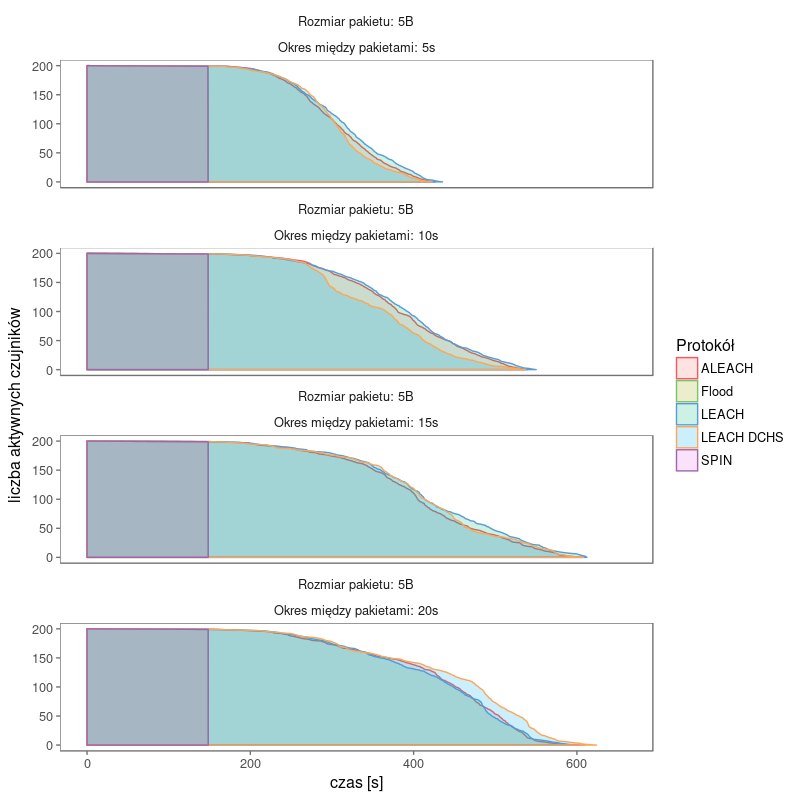
\includegraphics[scale=0.7]{\ImgPath/charts/alive_nodes_normal_200sensors_row1.png}
	\end{center}
	\caption{Aktywne węzły - 200 czujników, rozkład normalny, rozmiar pakietu: 5B}
\end{figure}

\begin{figure}[H]
	\begin{center}
		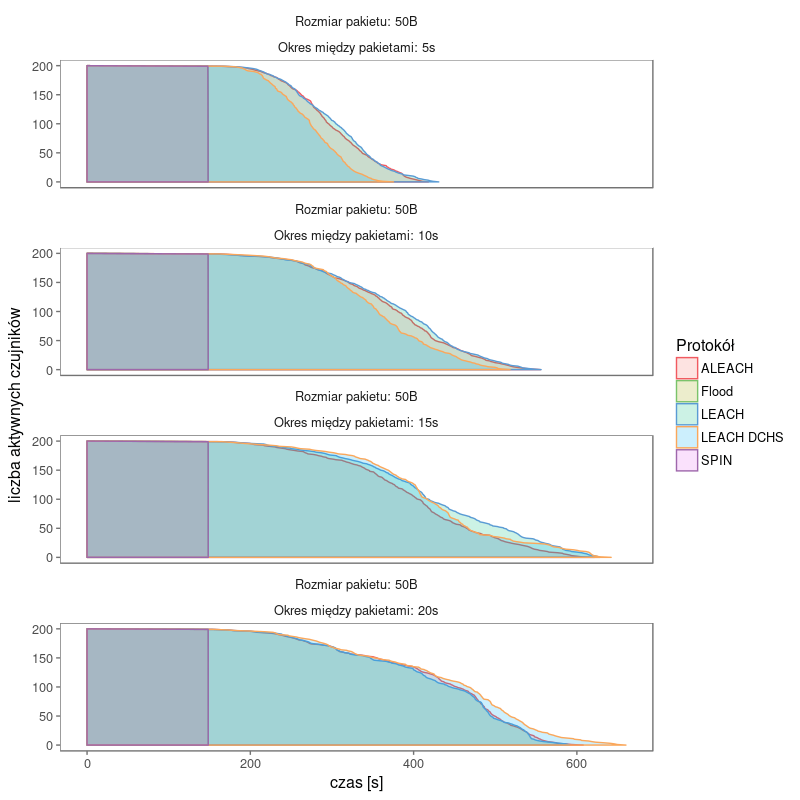
\includegraphics[scale=0.7]{\ImgPath/charts/alive_nodes_normal_200sensors_row2.png}
	\end{center}
	\caption{Aktywne węzły - 200 czujników, rozkład normalny, rozmiar pakietu: 50B}
\end{figure}

\begin{figure}[H]
	\begin{center}
		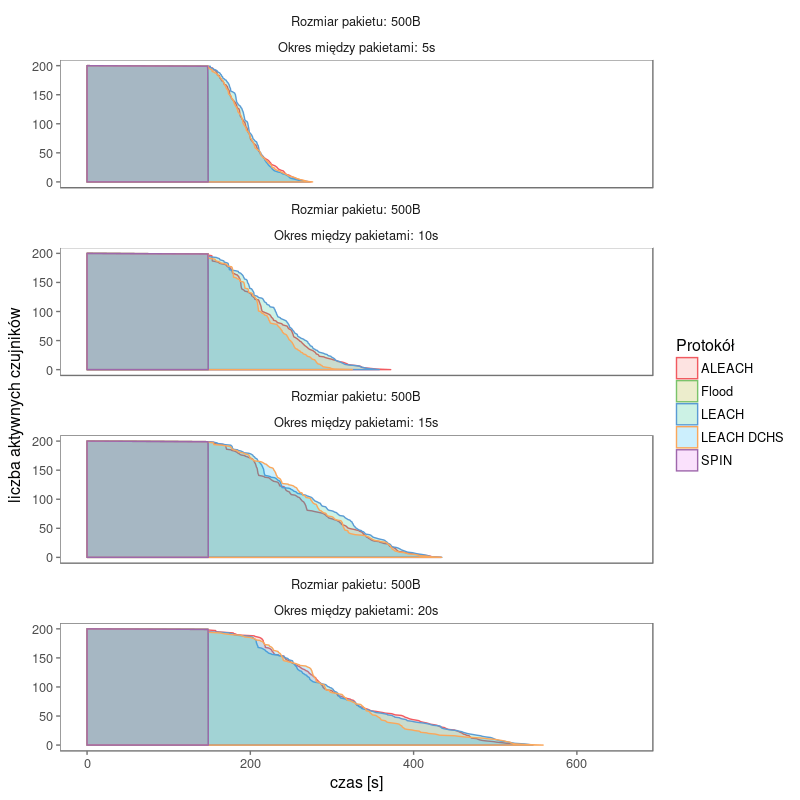
\includegraphics[scale=0.7]{\ImgPath/charts/alive_nodes_normal_200sensors_row3.png}
	\end{center}
	\caption{Aktywne węzły - 200 czujników, rozkład normalny, rozmiar pakietu: 500B}
\end{figure}

\begin{figure}[H]
	\begin{center}
		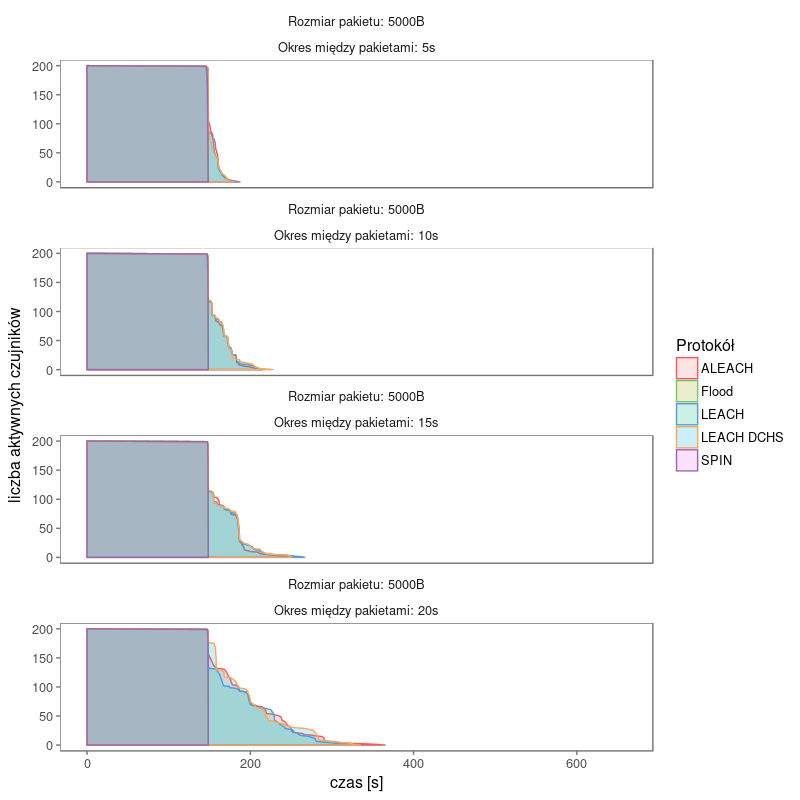
\includegraphics[scale=0.7]{\ImgPath/charts/alive_nodes_normal_200sensors_row4.png}
	\end{center}
	\caption{Aktywne węzły - 200 czujników, rozkład normalny, rozmiar pakietu: 5000B}
\end{figure}

\begin{figure}[H]
	\begin{center}
		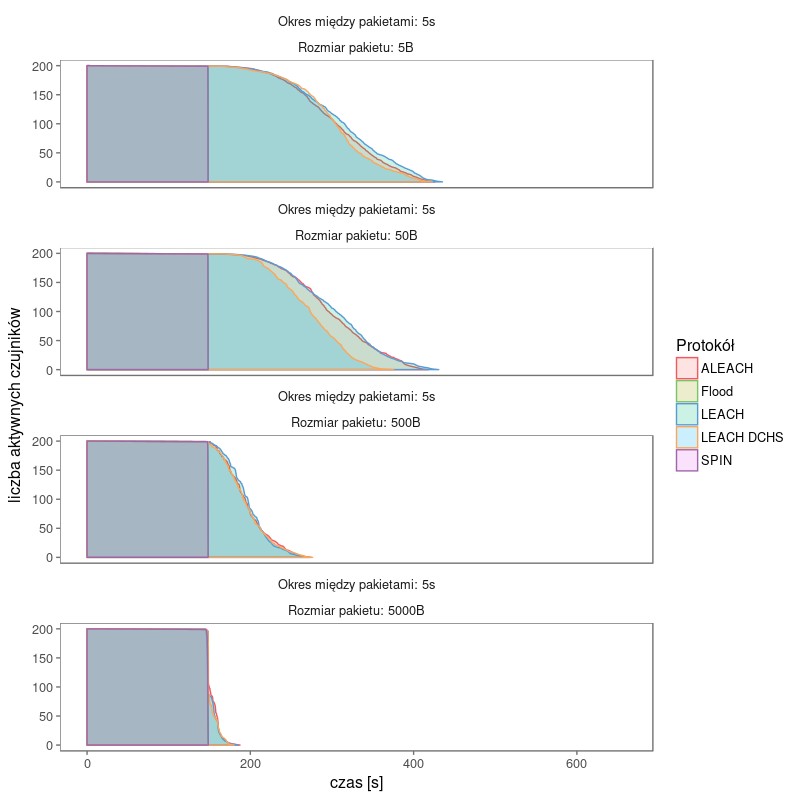
\includegraphics[scale=0.7]{\ImgPath/charts/alive_nodes_normal_200sensors_col1.png}
	\end{center}
	\caption{Aktywne węzły - 200 czujników, rozkład normalny, okres pomiędzy pakietami: 5s}
\end{figure}

\begin{figure}[H]
	\begin{center}
		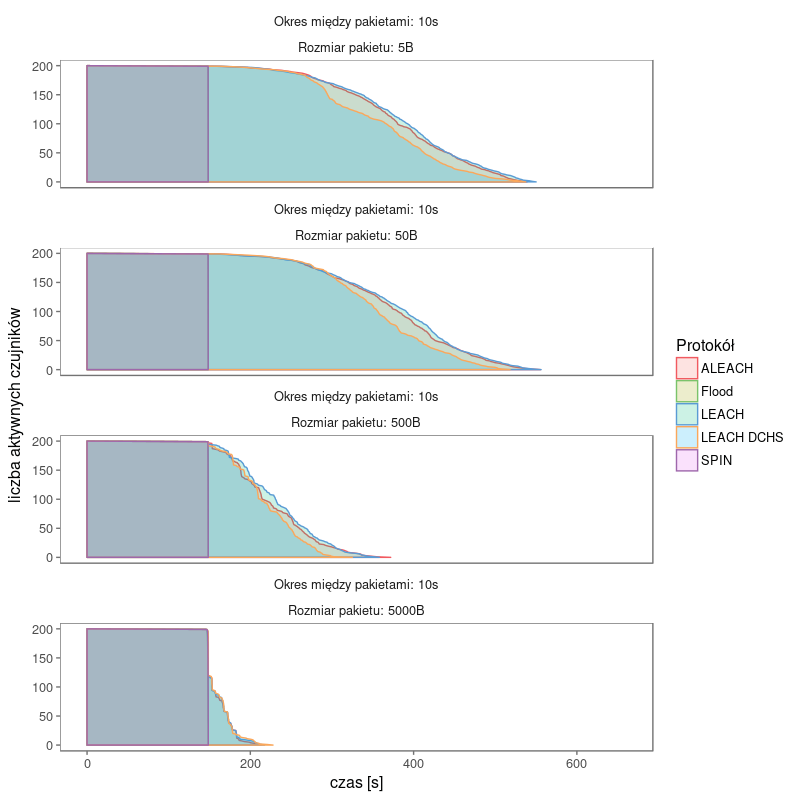
\includegraphics[scale=0.7]{\ImgPath/charts/alive_nodes_normal_200sensors_col2.png}
	\end{center}
	\caption{Aktywne węzły - 200 czujników, rozkład normalny, okres pomiędzy pakietami: 10s}
\end{figure}

\begin{figure}[H]
	\begin{center}
		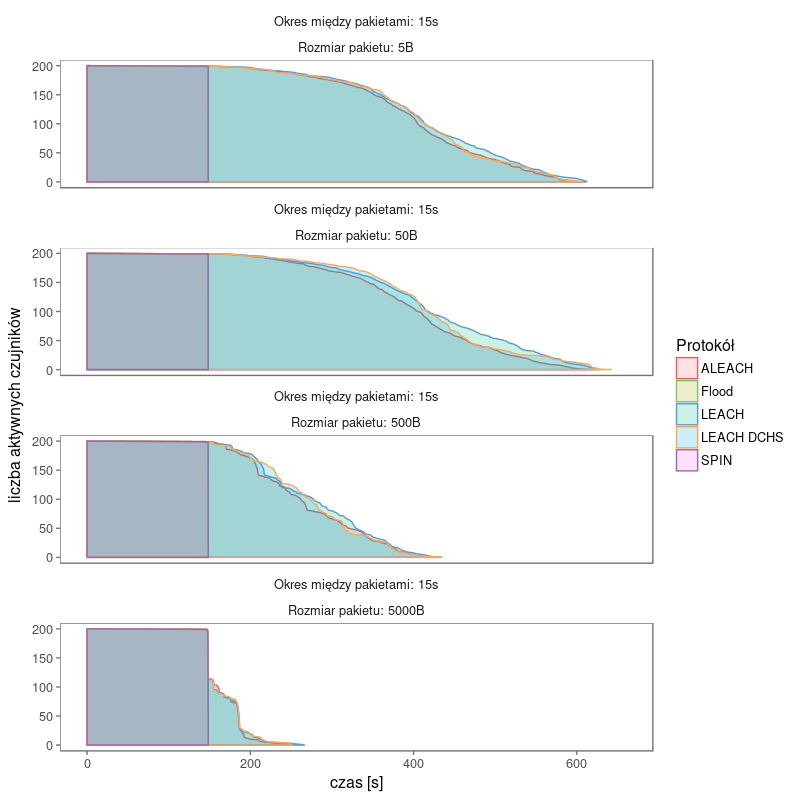
\includegraphics[scale=0.7]{\ImgPath/charts/alive_nodes_normal_200sensors_col3.png}
	\end{center}
	\caption{Aktywne węzły - 200 czujników, rozkład normalny, okres pomiędzy pakietami: 15s}
\end{figure}

\begin{figure}[H]
	\begin{center}
		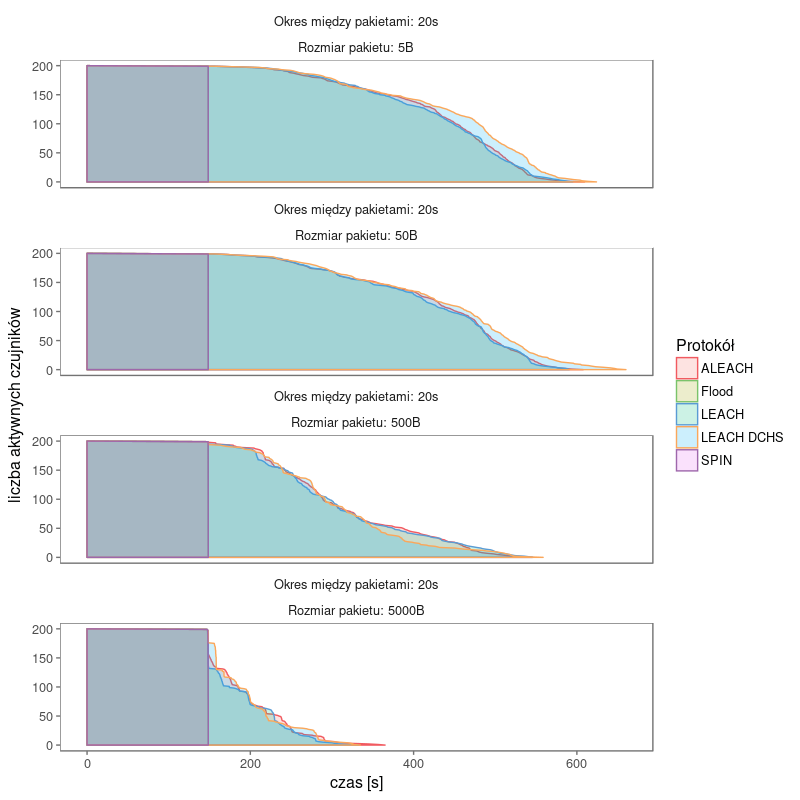
\includegraphics[scale=0.7]{\ImgPath/charts/alive_nodes_normal_200sensors_col4.png}
	\end{center}
	\caption{Aktywne węzły - 200 czujników, rozkład normalny, okres pomiędzy pakietami: 20s}
\end{figure}

\begin{figure}[H]
	\begin{center}
		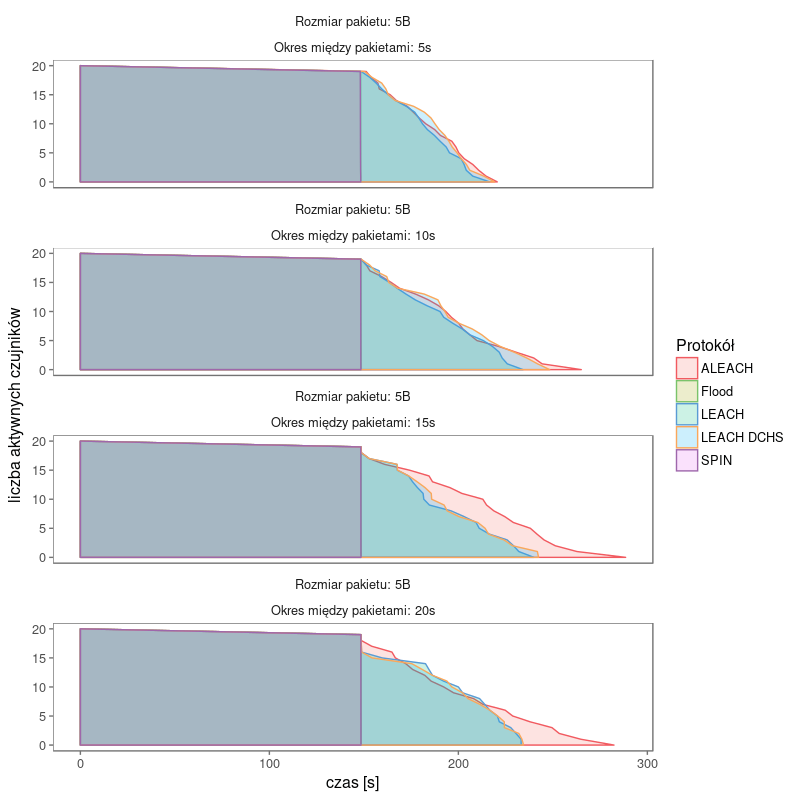
\includegraphics[scale=0.7]{\ImgPath/charts/alive_nodes_uniform_20sensors_row1.png}
	\end{center}
	\caption{Aktywne węzły - 20 czujników, rozkład jednorodny, rozmiar pakietu: 5B}
\end{figure}

\begin{figure}[H]
	\begin{center}
		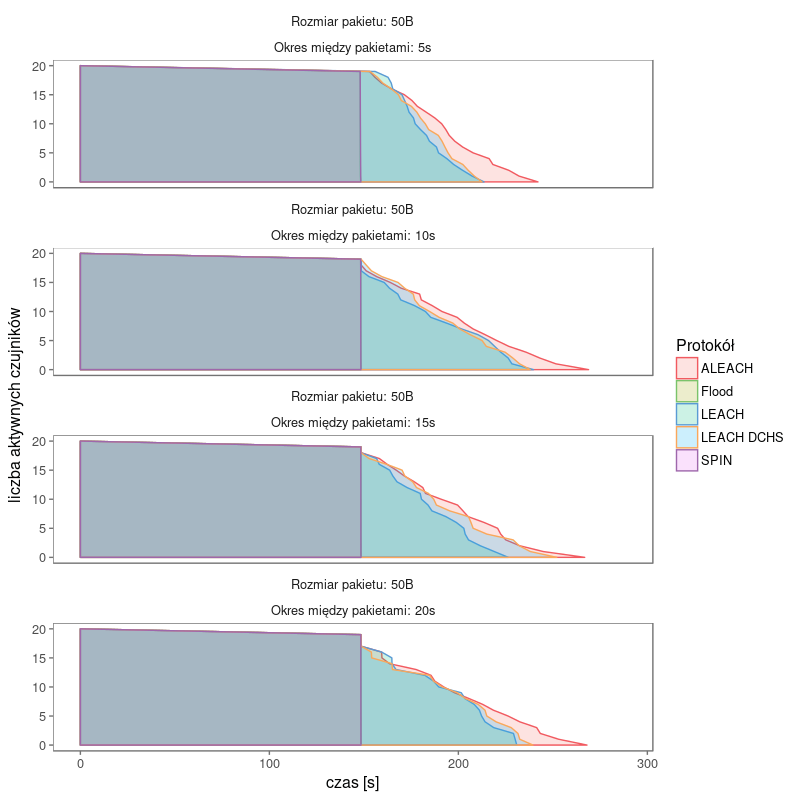
\includegraphics[scale=0.7]{\ImgPath/charts/alive_nodes_uniform_20sensors_row2.png}
	\end{center}
	\caption{Aktywne węzły - 20 czujników, rozkład jednorodny, rozmiar pakietu: 50B}
\end{figure}

\begin{figure}[H]
	\begin{center}
		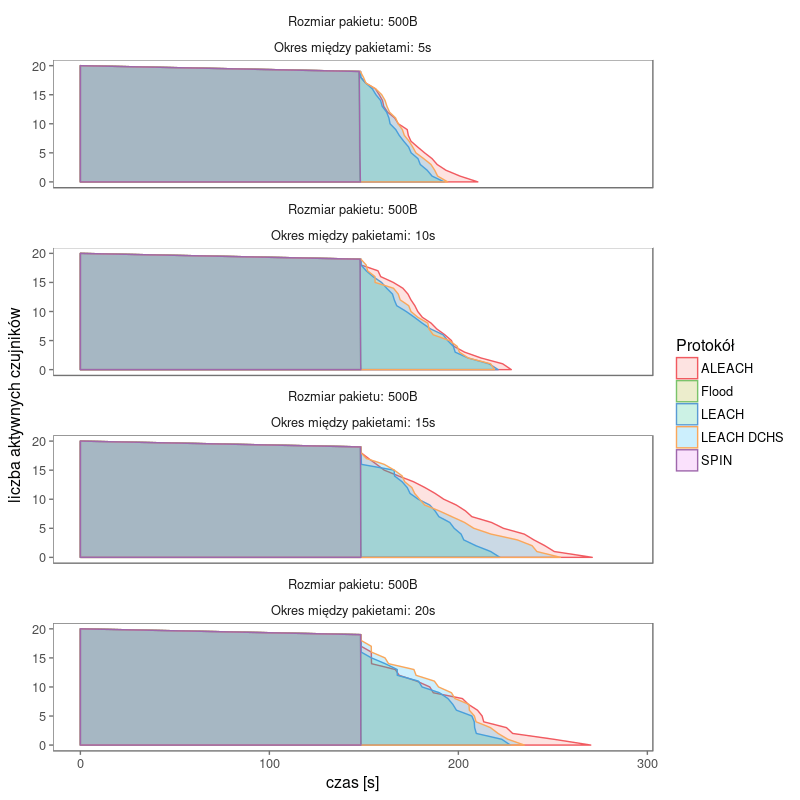
\includegraphics[scale=0.7]{\ImgPath/charts/alive_nodes_uniform_20sensors_row3.png}
	\end{center}
	\caption{Aktywne węzły - 20 czujników, rozkład jednorodny, rozmiar pakietu: 500B}
\end{figure}

\begin{figure}[H]
	\begin{center}
		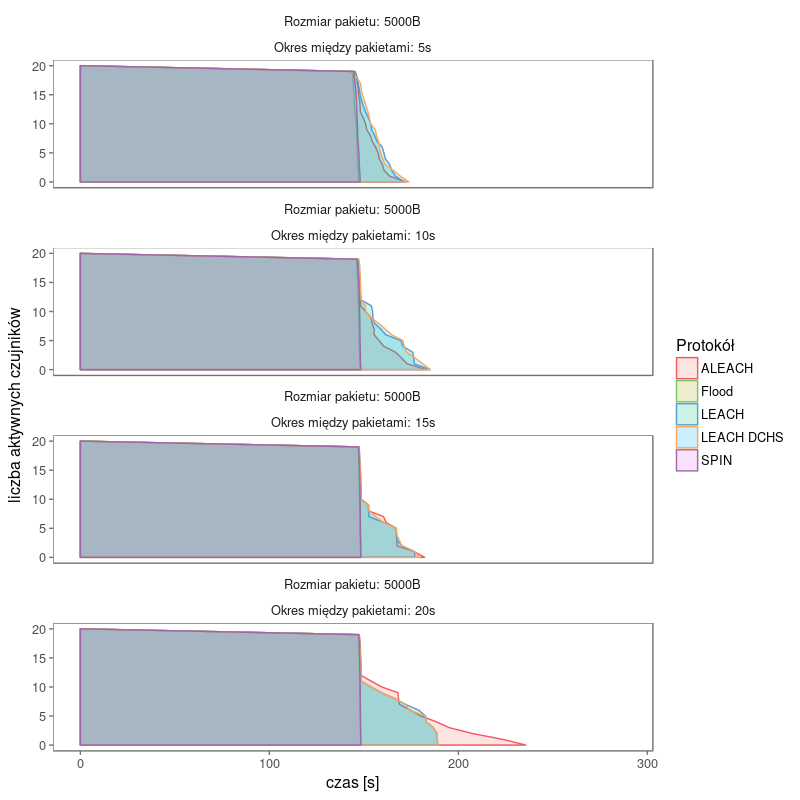
\includegraphics[scale=0.7]{\ImgPath/charts/alive_nodes_uniform_20sensors_row4.png}
	\end{center}
	\caption{Aktywne węzły - 20 czujników, rozkład jednorodny, rozmiar pakietu: 5000B}
\end{figure}

\begin{figure}[H]
	\begin{center}
		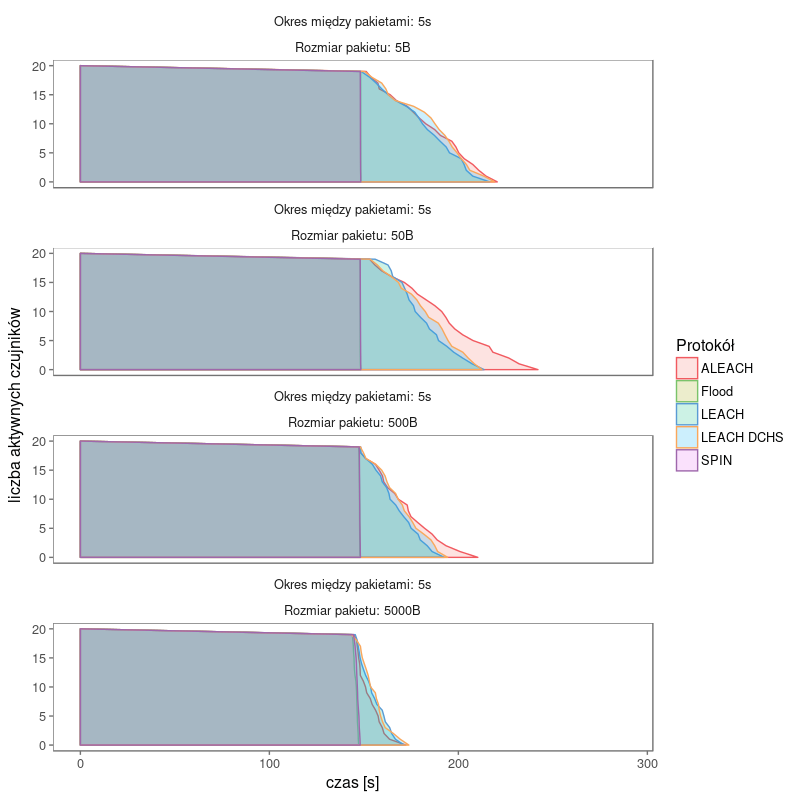
\includegraphics[scale=0.7]{\ImgPath/charts/alive_nodes_uniform_20sensors_col1.png}
	\end{center}
	\caption{Aktywne węzły - 20 czujników, rozkład jednorodny, okres pomiędzy pakietami: 5s}
\end{figure}

\begin{figure}[H]
	\begin{center}
		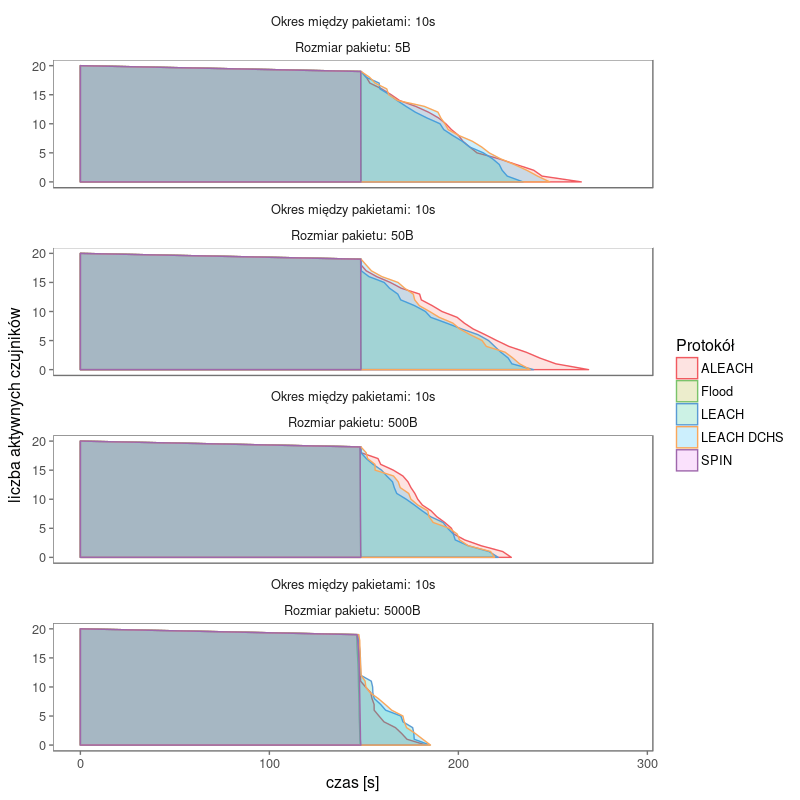
\includegraphics[scale=0.7]{\ImgPath/charts/alive_nodes_uniform_20sensors_col2.png}
	\end{center}
	\caption{Aktywne węzły - 20 czujników, rozkład jednorodny, okres pomiędzy pakietami: 10s}
\end{figure}

\begin{figure}[H]
	\begin{center}
		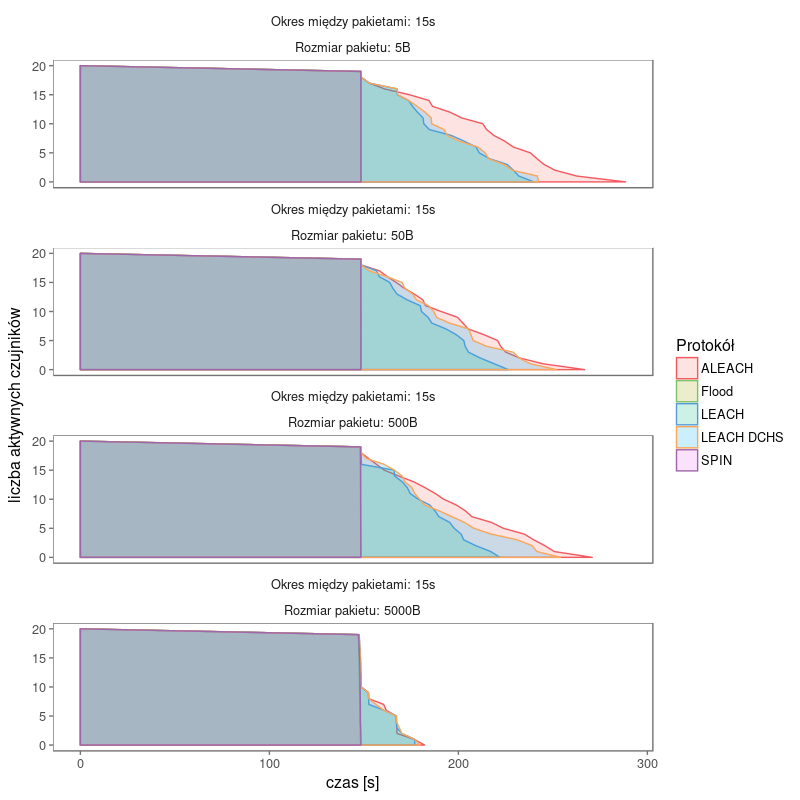
\includegraphics[scale=0.7]{\ImgPath/charts/alive_nodes_uniform_20sensors_col3.png}
	\end{center}
	\caption{Aktywne węzły - 20 czujników, rozkład jednorodny, okres pomiędzy pakietami: 15s}
\end{figure}

\begin{figure}[H]
	\begin{center}
		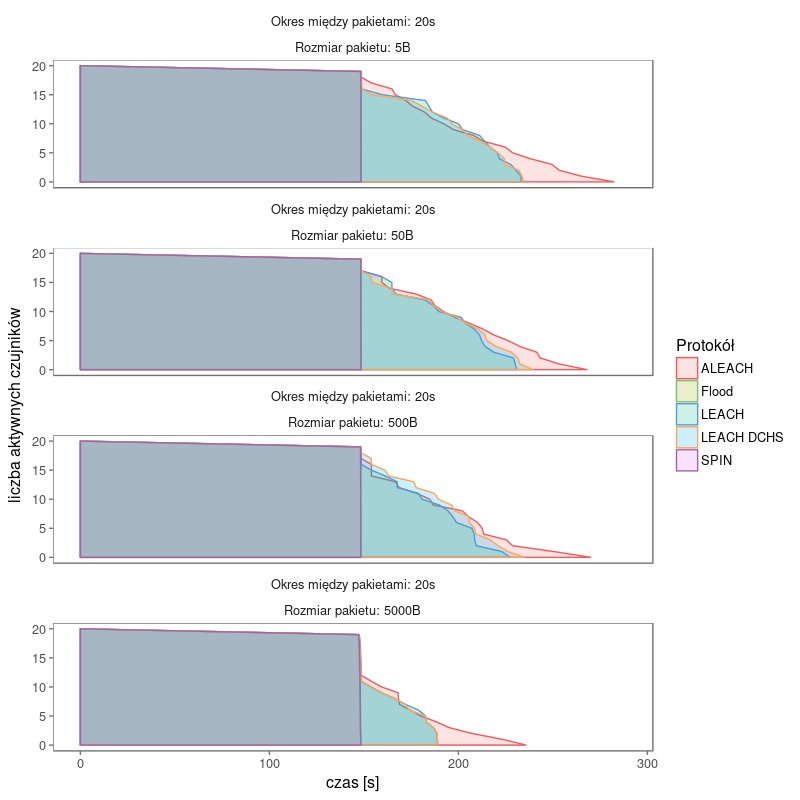
\includegraphics[scale=0.7]{\ImgPath/charts/alive_nodes_uniform_20sensors_col4.png}
	\end{center}
	\caption{Aktywne węzły - 20 czujników, rozkład jednorodny, okres pomiędzy pakietami: 20s}
\end{figure}

\begin{figure}[H]
	\begin{center}
		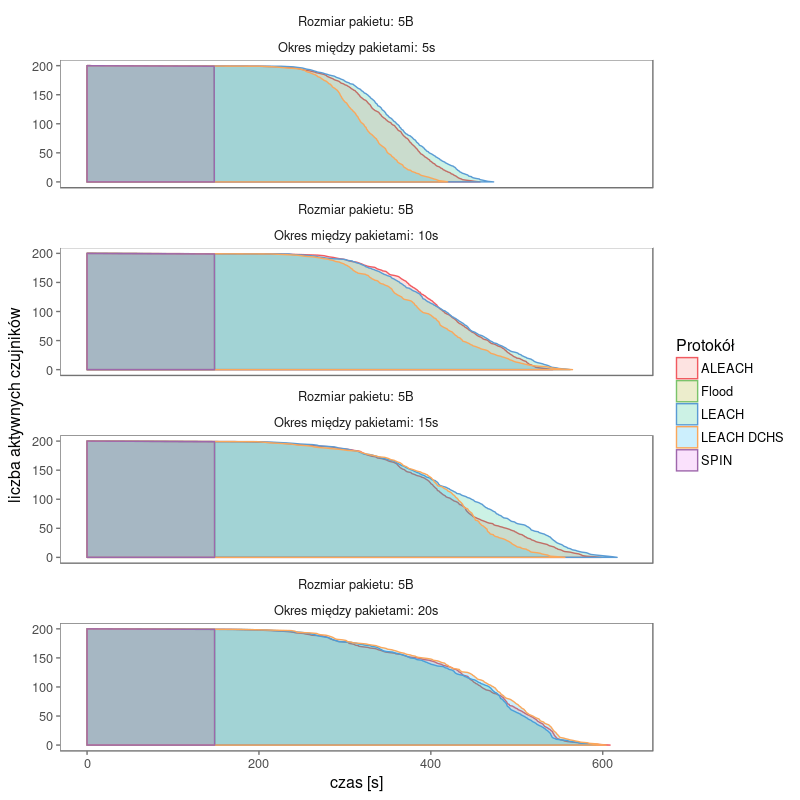
\includegraphics[scale=0.7]{\ImgPath/charts/alive_nodes_uniform_200sensors_row1.png}
	\end{center}
	\caption{Aktywne węzły - 200 czujników, rozkład jednorodny, rozmiar pakietu: 5B}
\end{figure}

\begin{figure}[H]
	\begin{center}
		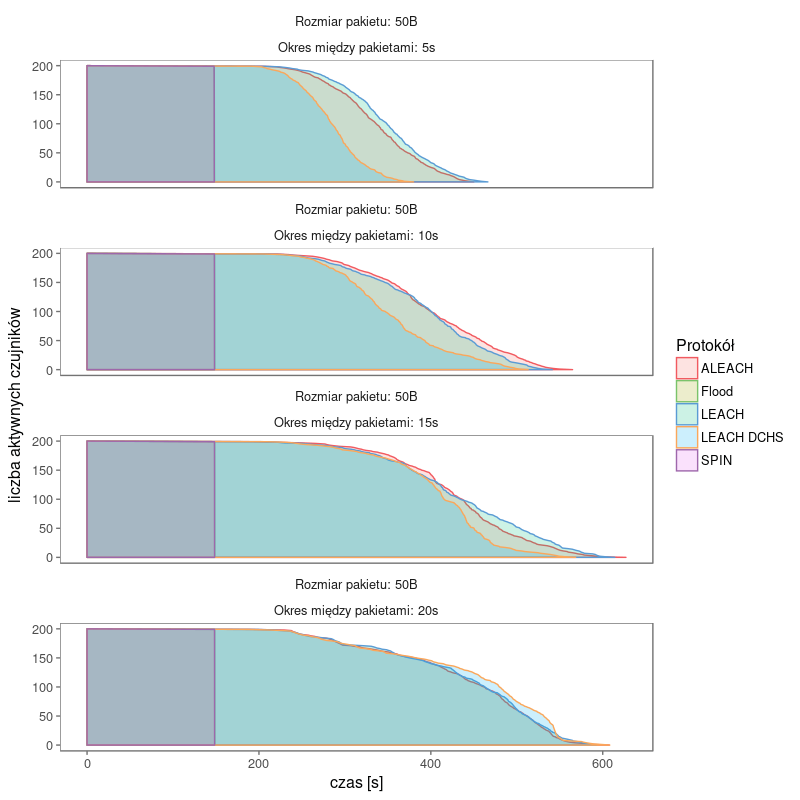
\includegraphics[scale=0.7]{\ImgPath/charts/alive_nodes_uniform_200sensors_row2.png}
	\end{center}
	\caption{Aktywne węzły - 200 czujników, rozkład jednorodny, rozmiar pakietu: 50B}
\end{figure}

\begin{figure}[H]
	\begin{center}
		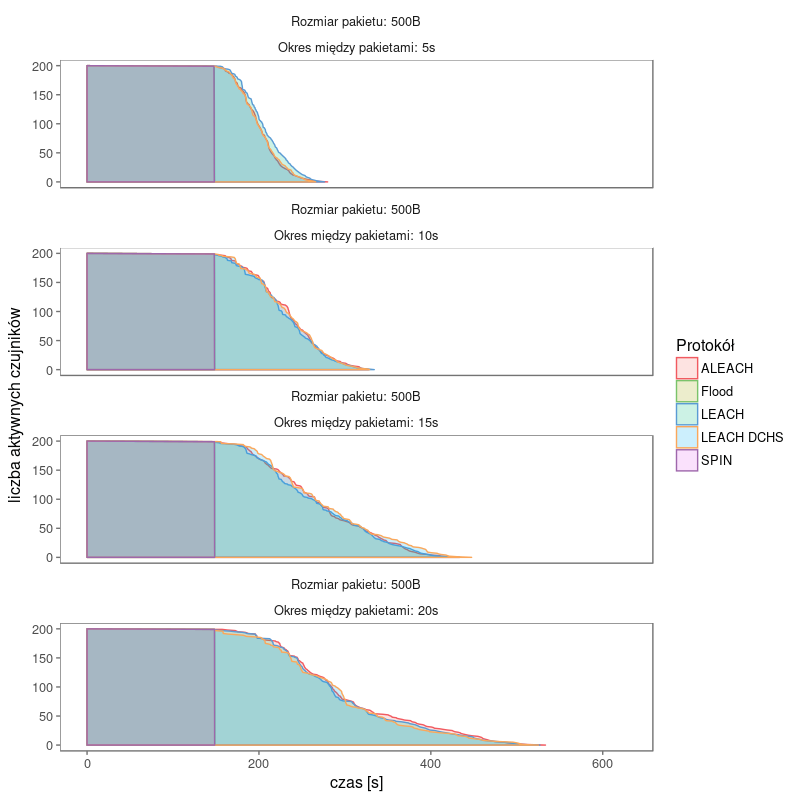
\includegraphics[scale=0.7]{\ImgPath/charts/alive_nodes_uniform_200sensors_row3.png}
	\end{center}
	\caption{Aktywne węzły - 200 czujników, rozkład jednorodny, rozmiar pakietu: 500B}
\end{figure}

\begin{figure}[H]
	\begin{center}
		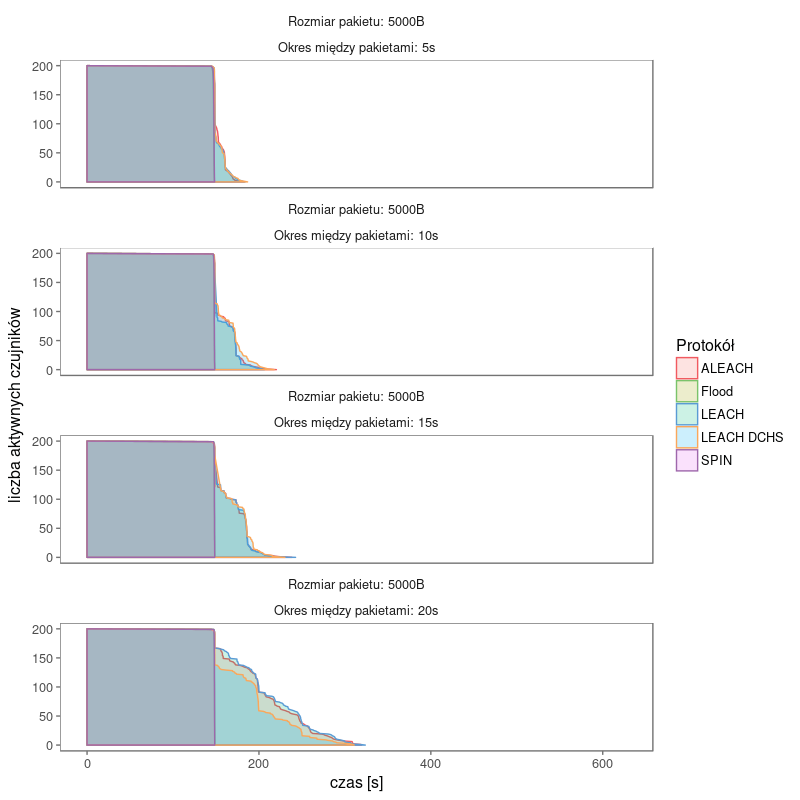
\includegraphics[scale=0.7]{\ImgPath/charts/alive_nodes_uniform_200sensors_row4.png}
	\end{center}
	\caption{Aktywne węzły - 200 czujników, rozkład jednorodny, rozmiar pakietu: 5000B}
\end{figure}

\begin{figure}[H]
	\begin{center}
		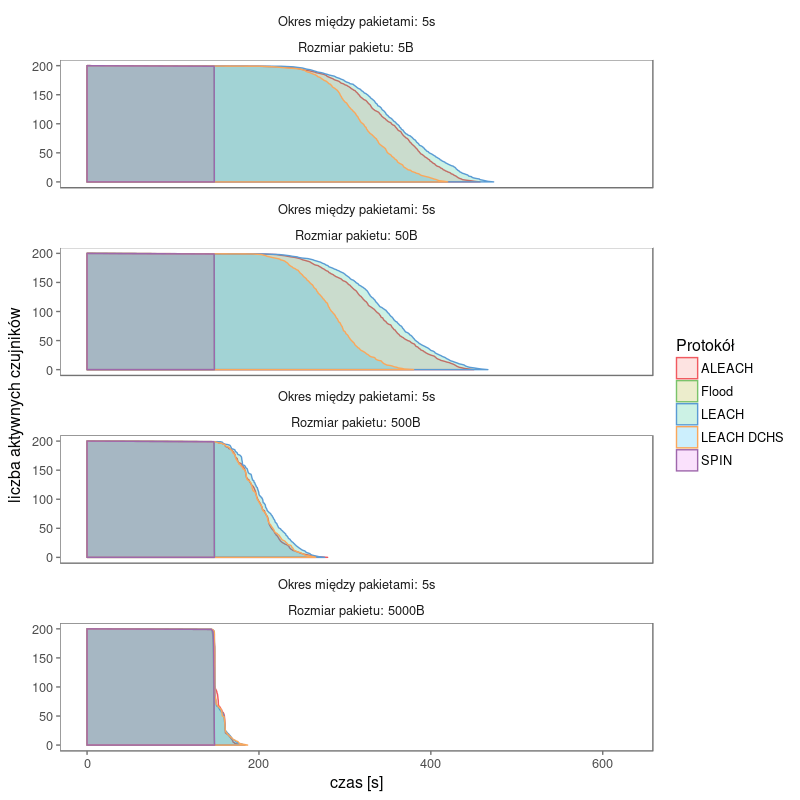
\includegraphics[scale=0.7]{\ImgPath/charts/alive_nodes_uniform_200sensors_col1.png}
	\end{center}
	\caption{Aktywne węzły - 200 czujników, rozkład jednorodny, okres pomiędzy pakietami: 5s}
\end{figure}

\begin{figure}[H]
	\begin{center}
		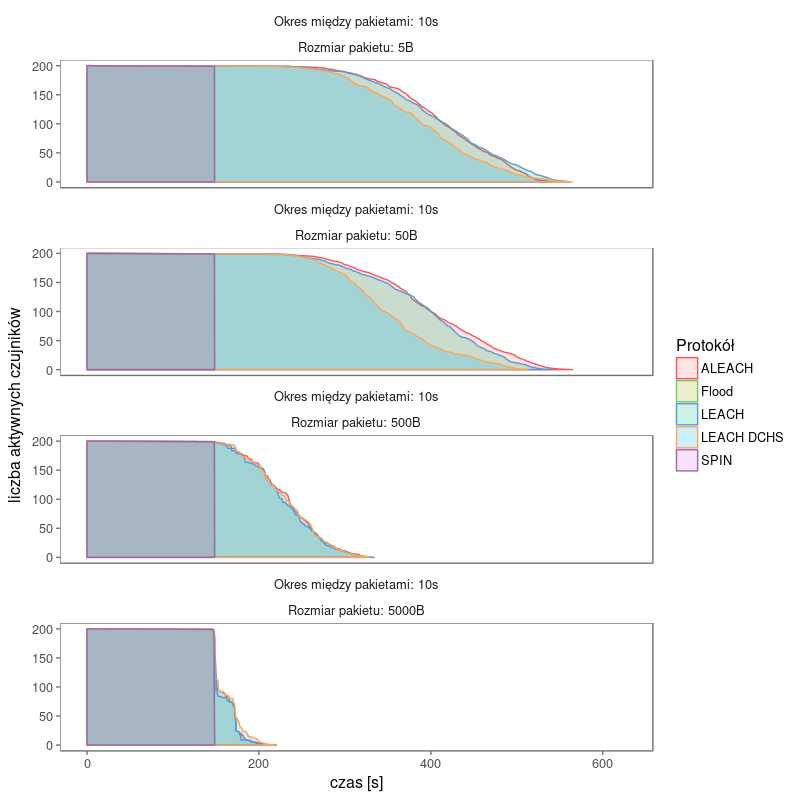
\includegraphics[scale=0.7]{\ImgPath/charts/alive_nodes_uniform_200sensors_col2.png}
	\end{center}
	\caption{Aktywne węzły - 200 czujników, rozkład jednorodny, okres pomiędzy pakietami: 10s}
\end{figure}

\begin{figure}[H]
	\begin{center}
		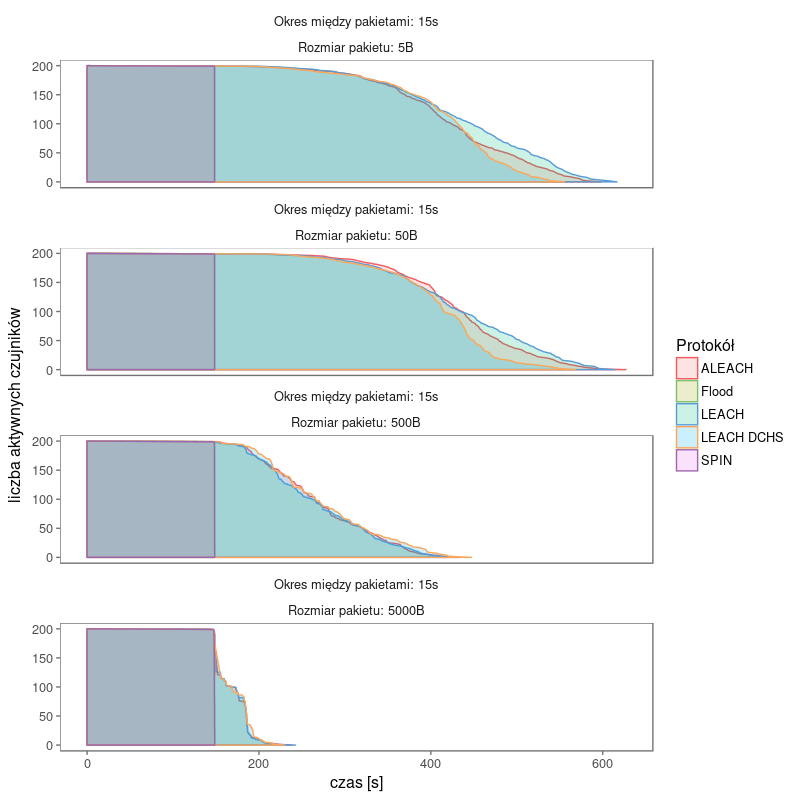
\includegraphics[scale=0.7]{\ImgPath/charts/alive_nodes_uniform_200sensors_col3.png}
	\end{center}
	\caption{Aktywne węzły - 200 czujników, rozkład jednorodny, okres pomiędzy pakietami: 15s}
\end{figure}

\begin{figure}[H]
	\begin{center}
		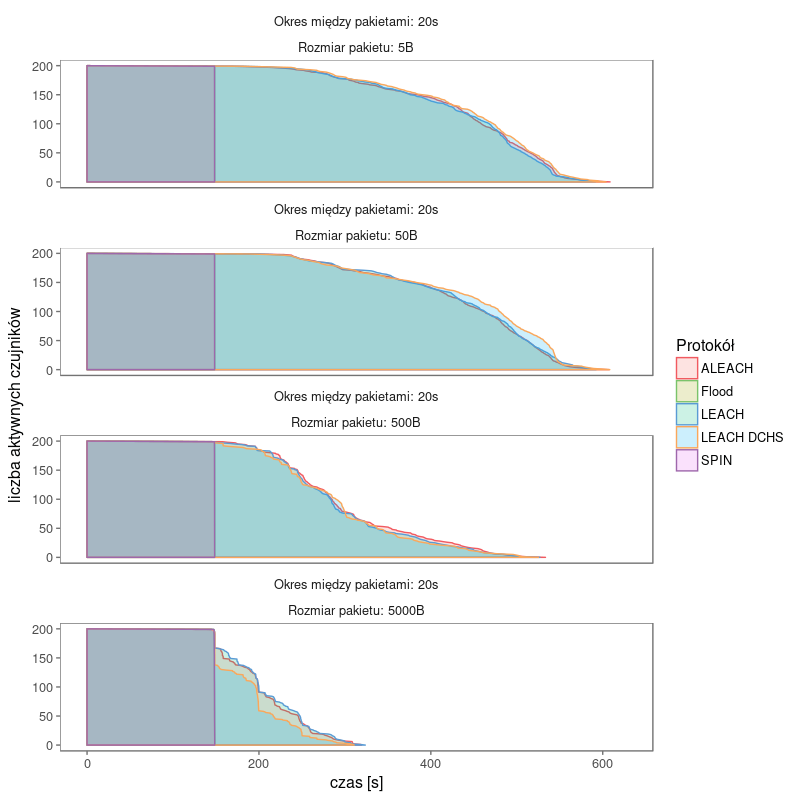
\includegraphics[scale=0.7]{\ImgPath/charts/alive_nodes_uniform_200sensors_col4.png}
	\end{center}
	\caption{Aktywne węzły - 200 czujników, rozkład jednorodny, okres pomiędzy pakietami: 20s}
\end{figure}

\begin{figure}[H]
	\begin{center}
		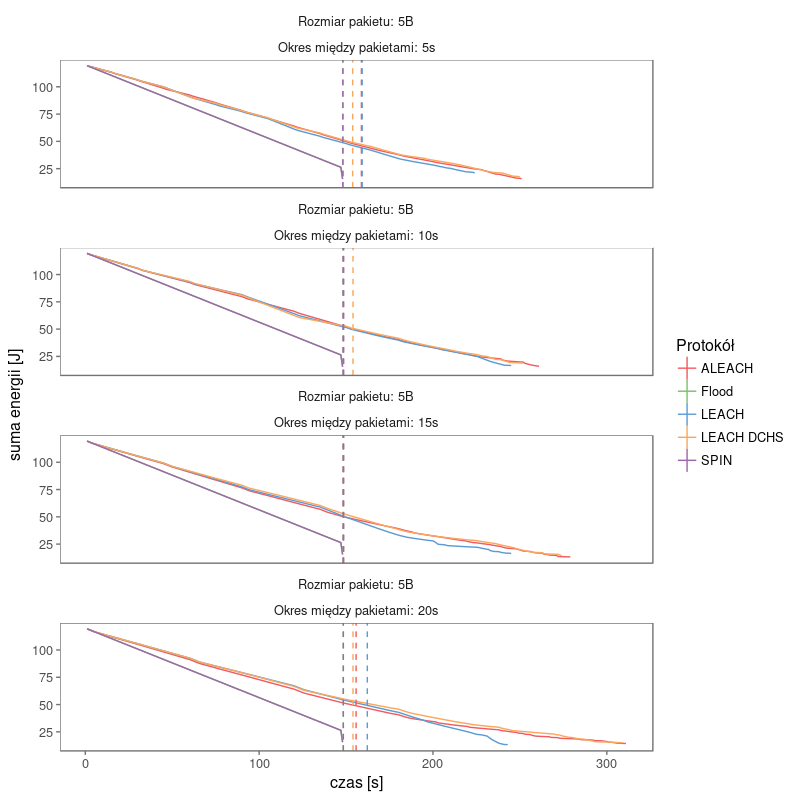
\includegraphics[scale=0.7]{\ImgPath/charts/stored_energy_normal_20sensors_row1.png}
	\end{center}
	\caption{Energia sieci - 20 czujników, rozkład normalny, rozmiar pakietu: 5B}
\end{figure}

\begin{figure}[H]
	\begin{center}
		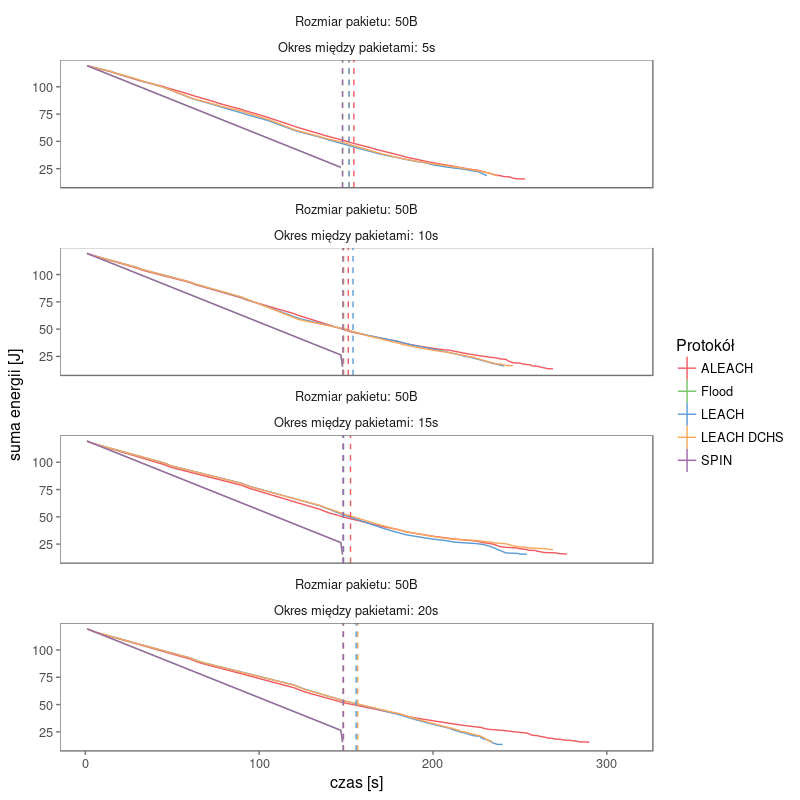
\includegraphics[scale=0.7]{\ImgPath/charts/stored_energy_normal_20sensors_row2.png}
	\end{center}
	\caption{Energia sieci - 20 czujników, rozkład normalny, rozmiar pakietu: 50B}
\end{figure}

\begin{figure}[H]
	\begin{center}
		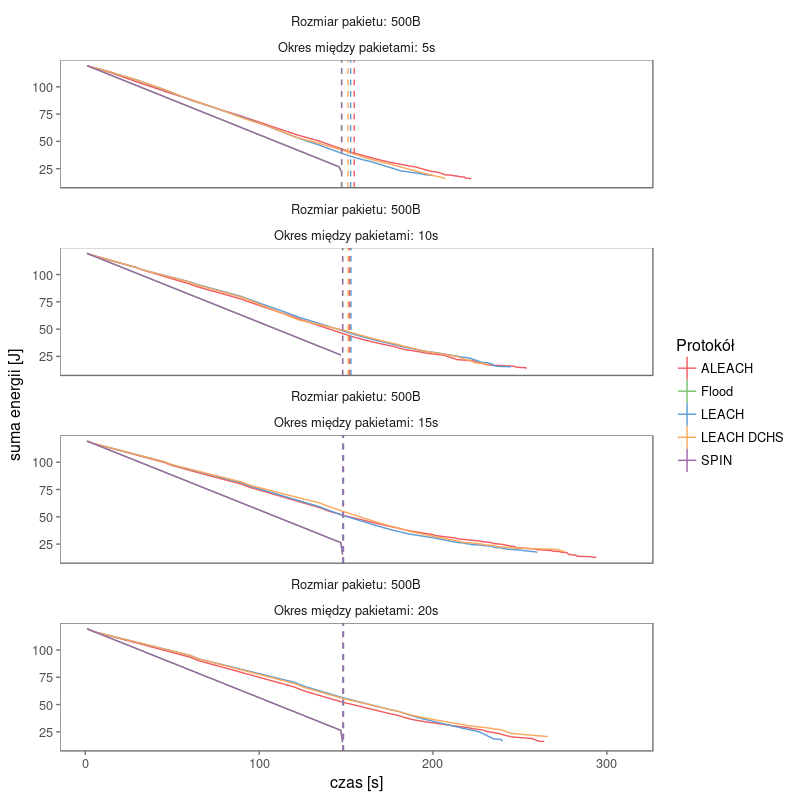
\includegraphics[scale=0.7]{\ImgPath/charts/stored_energy_normal_20sensors_row3.png}
	\end{center}
	\caption{Energia sieci - 20 czujników, rozkład normalny, rozmiar pakietu: 500B}
\end{figure}

\begin{figure}[H]
	\begin{center}
		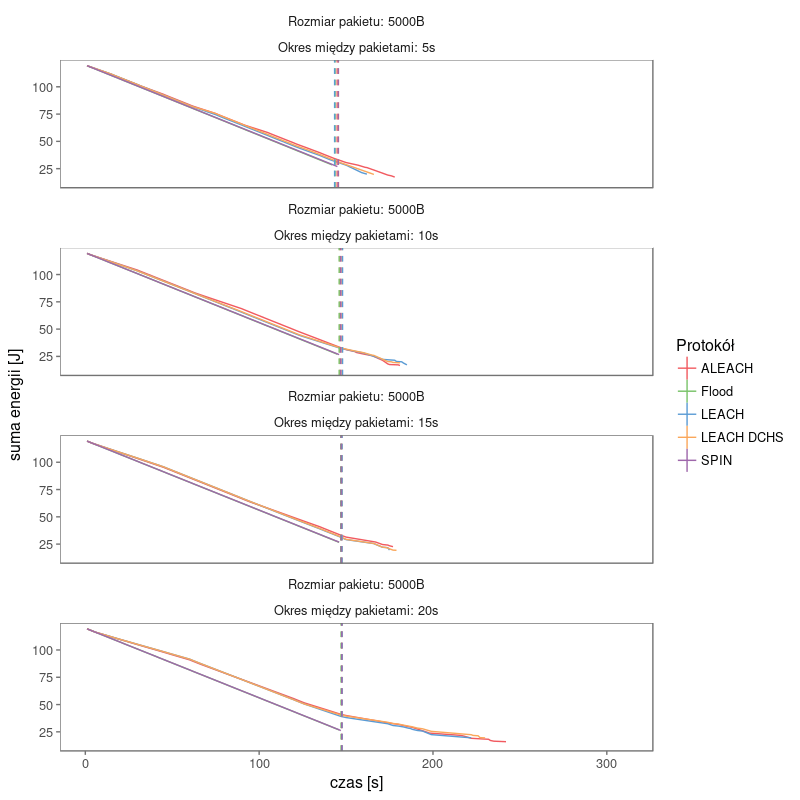
\includegraphics[scale=0.7]{\ImgPath/charts/stored_energy_normal_20sensors_row4.png}
	\end{center}
	\caption{Energia sieci - 20 czujników, rozkład normalny, rozmiar pakietu: 5000B}
\end{figure}

\begin{figure}[H]
	\begin{center}
		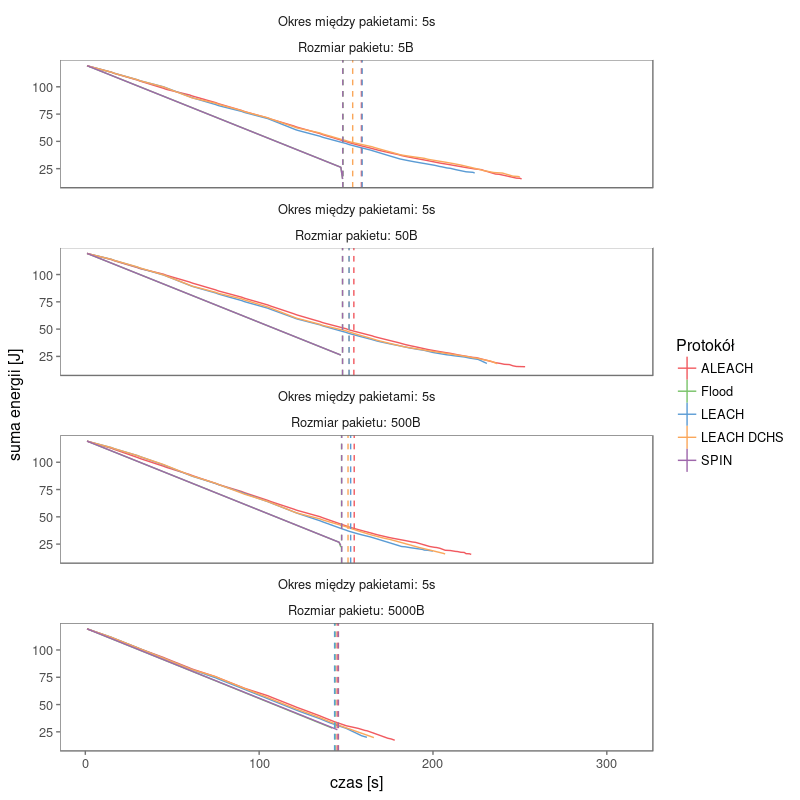
\includegraphics[scale=0.7]{\ImgPath/charts/stored_energy_normal_20sensors_col1.png}
	\end{center}
	\caption{Energia sieci - 20 czujników, rozkład normalny, okres pomiędzy pakietami: 5s}
\end{figure}

\begin{figure}[H]
	\begin{center}
		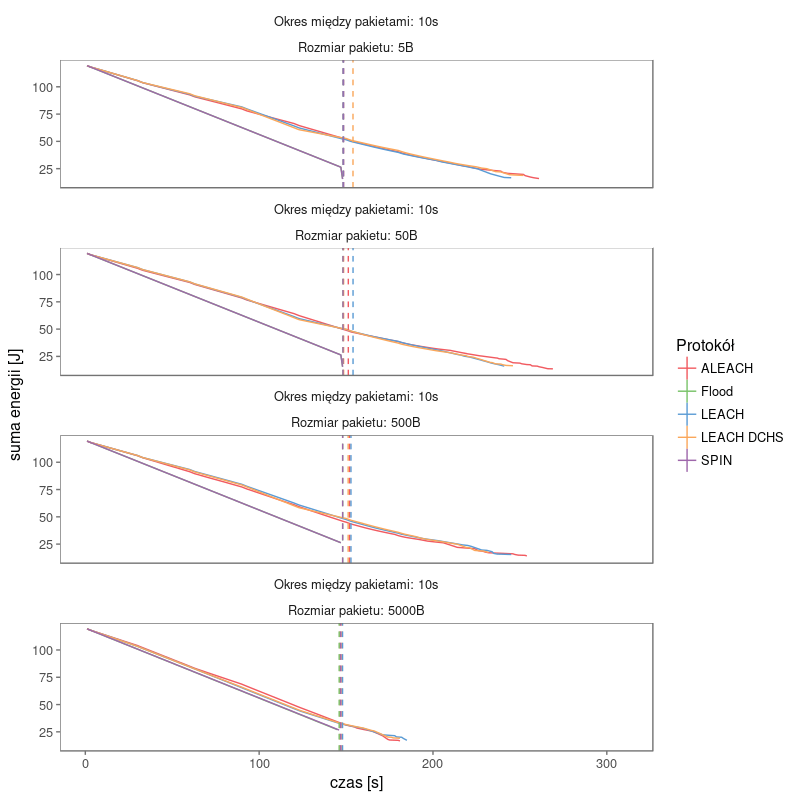
\includegraphics[scale=0.7]{\ImgPath/charts/stored_energy_normal_20sensors_col2.png}
	\end{center}
	\caption{Energia sieci - 20 czujników, rozkład normalny, okres pomiędzy pakietami: 10s}
\end{figure}

\begin{figure}[H]
	\begin{center}
		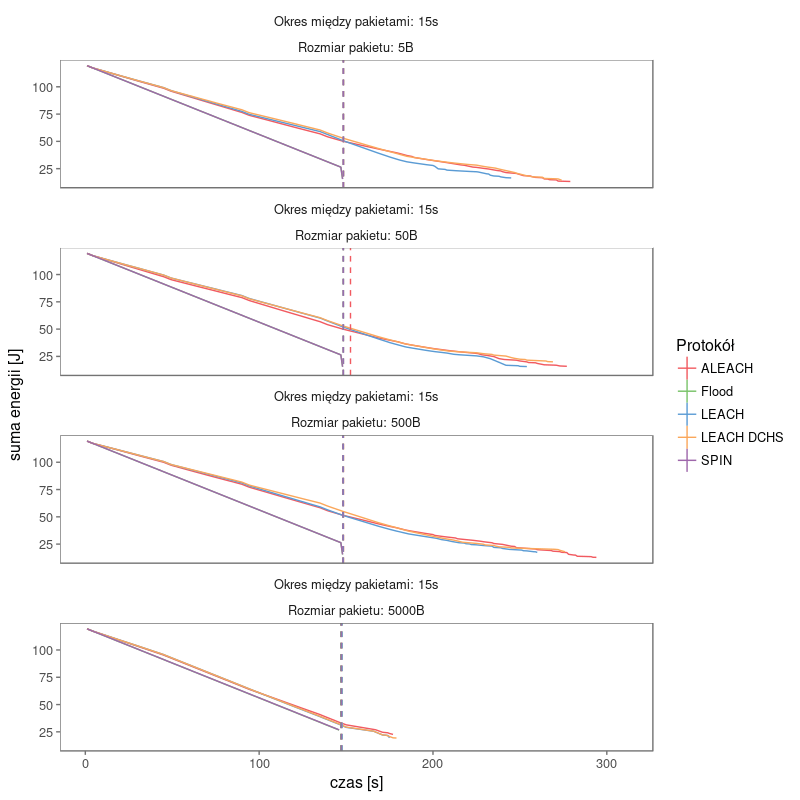
\includegraphics[scale=0.7]{\ImgPath/charts/stored_energy_normal_20sensors_col3.png}
	\end{center}
	\caption{Energia sieci - 20 czujników, rozkład normalny, okres pomiędzy pakietami: 15s}
\end{figure}

\begin{figure}[H]
	\begin{center}
		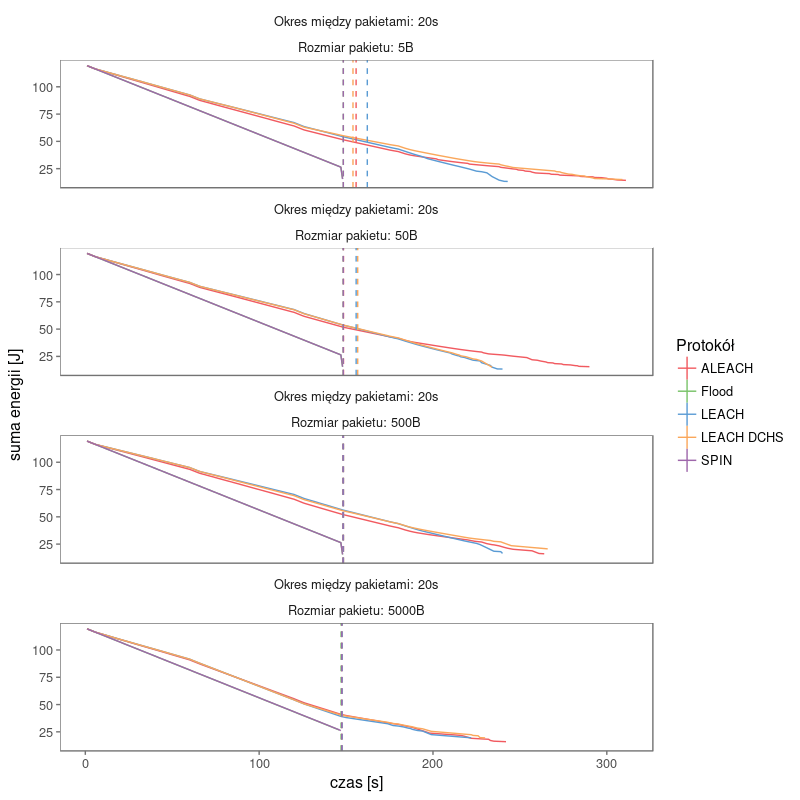
\includegraphics[scale=0.7]{\ImgPath/charts/stored_energy_normal_20sensors_col4.png}
	\end{center}
	\caption{Energia sieci - 20 czujników, rozkład normalny, okres pomiędzy pakietami: 20s}
\end{figure}

\begin{figure}[H]
	\begin{center}
		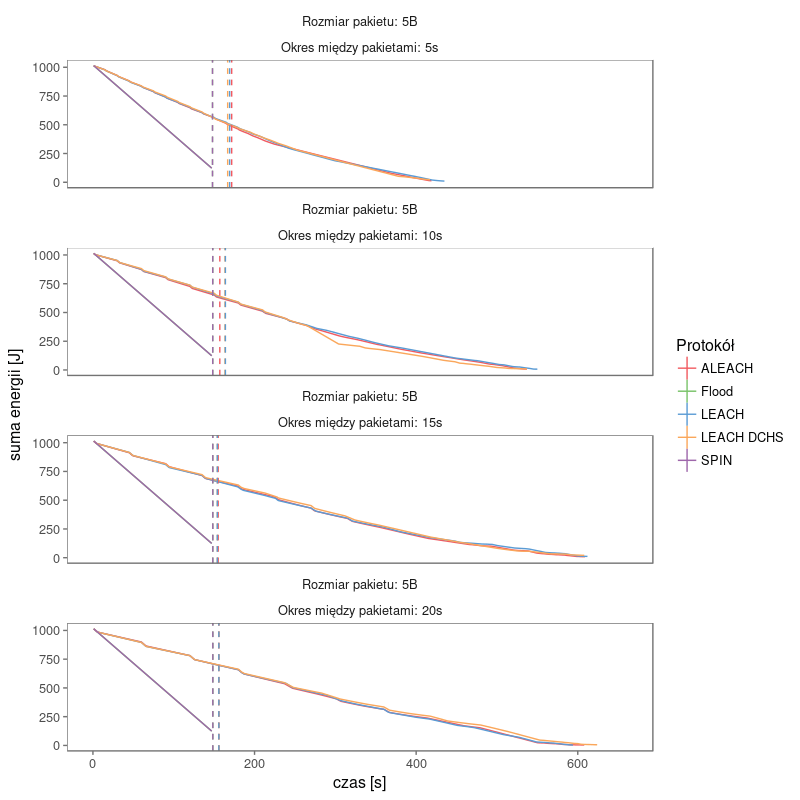
\includegraphics[scale=0.7]{\ImgPath/charts/stored_energy_normal_200sensors_row1.png}
	\end{center}
	\caption{Energia sieci - 200 czujników, rozkład normalny, rozmiar pakietu: 5B}
\end{figure}

\begin{figure}[H]
	\begin{center}
		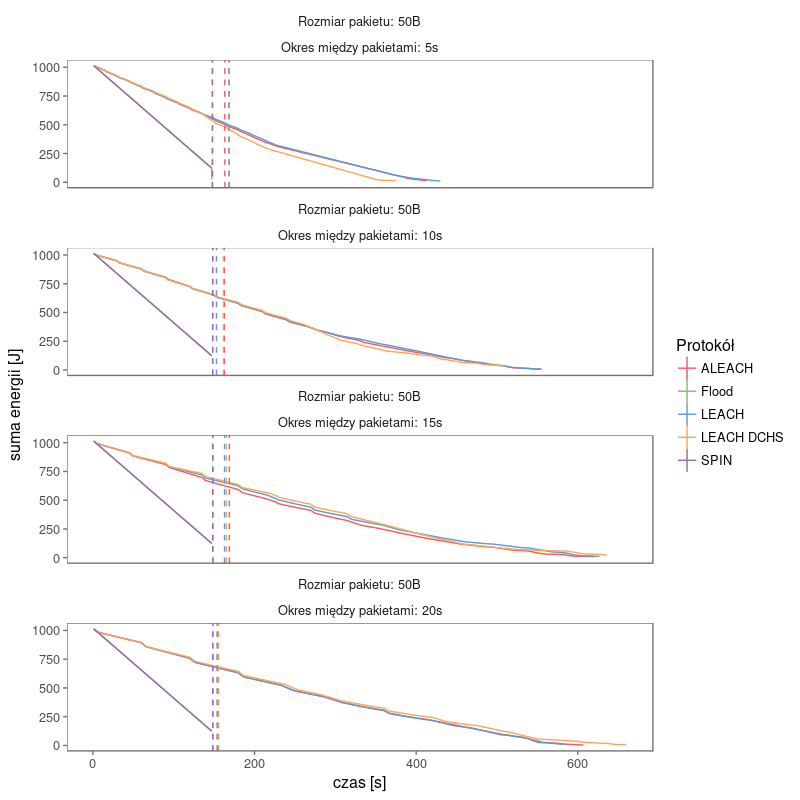
\includegraphics[scale=0.7]{\ImgPath/charts/stored_energy_normal_200sensors_row2.png}
	\end{center}
	\caption{Energia sieci - 200 czujników, rozkład normalny, rozmiar pakietu: 50B}
\end{figure}

\begin{figure}[H]
	\begin{center}
		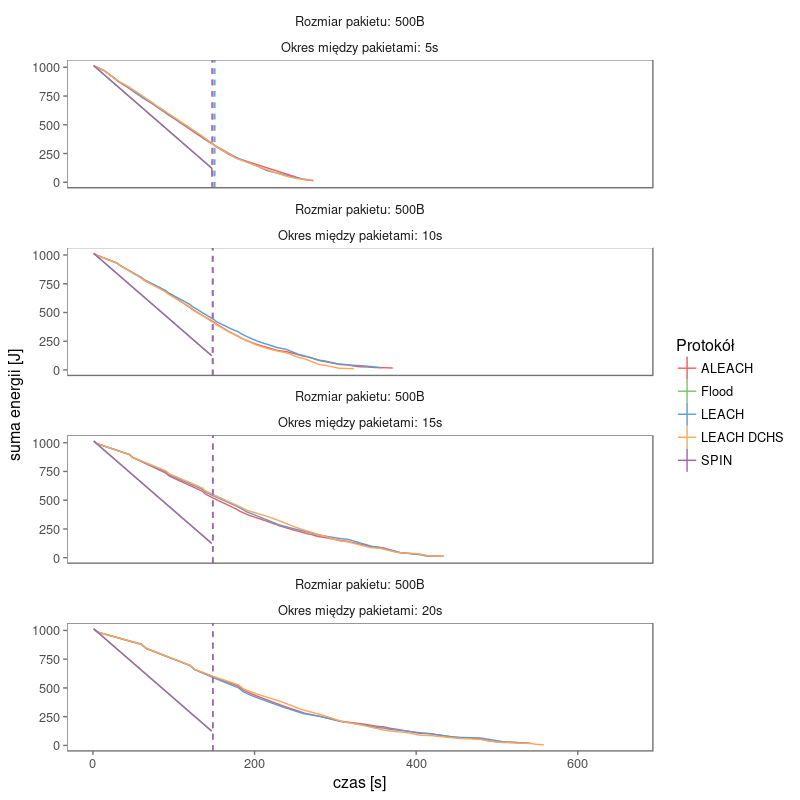
\includegraphics[scale=0.7]{\ImgPath/charts/stored_energy_normal_200sensors_row3.png}
	\end{center}
	\caption{Energia sieci - 200 czujników, rozkład normalny, rozmiar pakietu: 500B}
\end{figure}

\begin{figure}[H]
	\begin{center}
		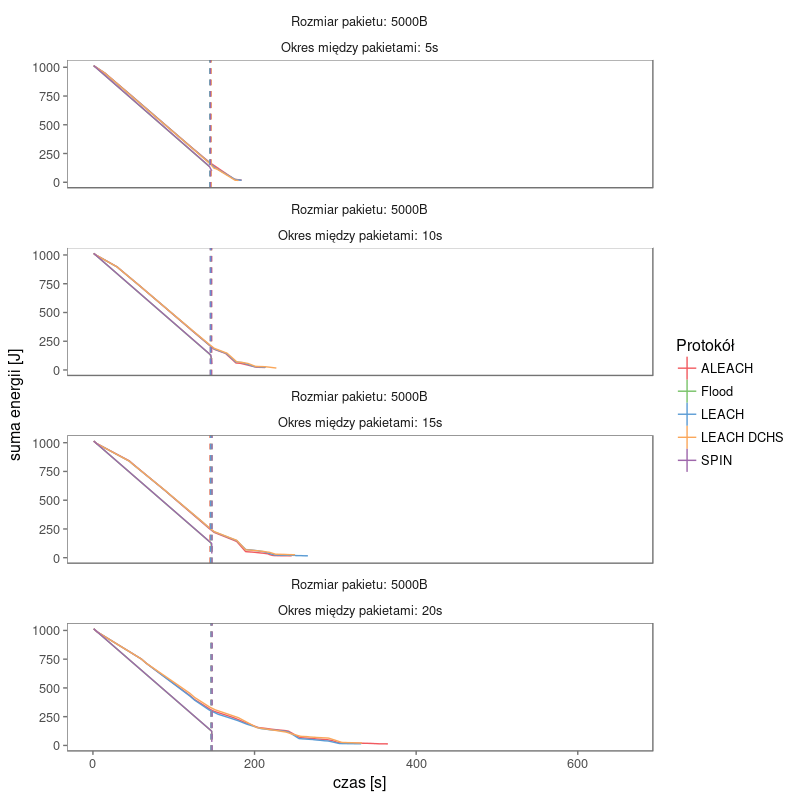
\includegraphics[scale=0.7]{\ImgPath/charts/stored_energy_normal_200sensors_row4.png}
	\end{center}
	\caption{Energia sieci - 200 czujników, rozkład normalny, rozmiar pakietu: 5000B}
\end{figure}

\begin{figure}[H]
	\begin{center}
		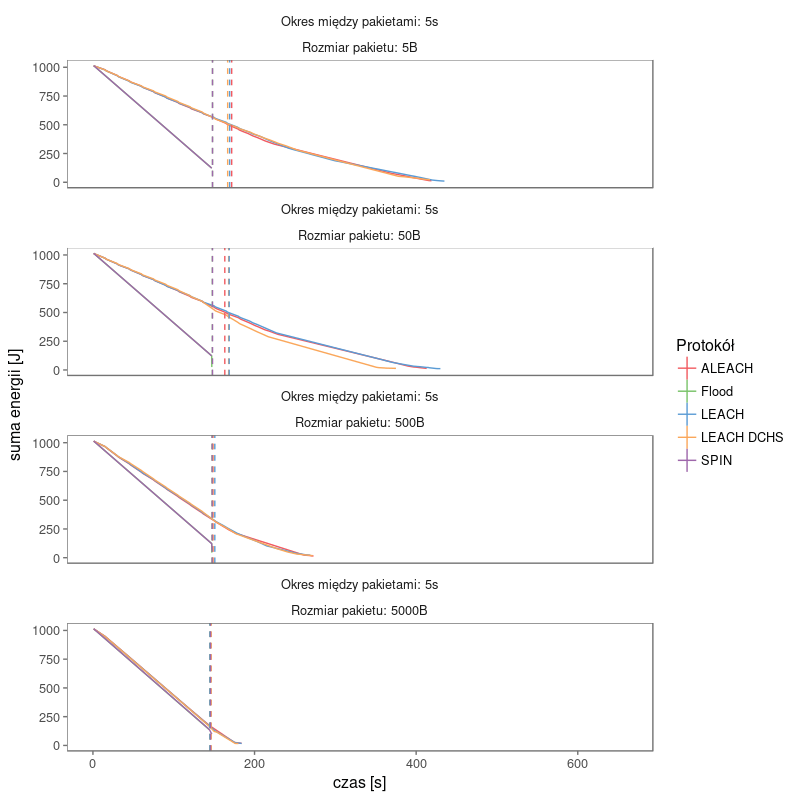
\includegraphics[scale=0.7]{\ImgPath/charts/stored_energy_normal_200sensors_col1.png}
	\end{center}
	\caption{Energia sieci - 200 czujników, rozkład normalny, okres pomiędzy pakietami: 5s}
\end{figure}

\begin{figure}[H]
	\begin{center}
		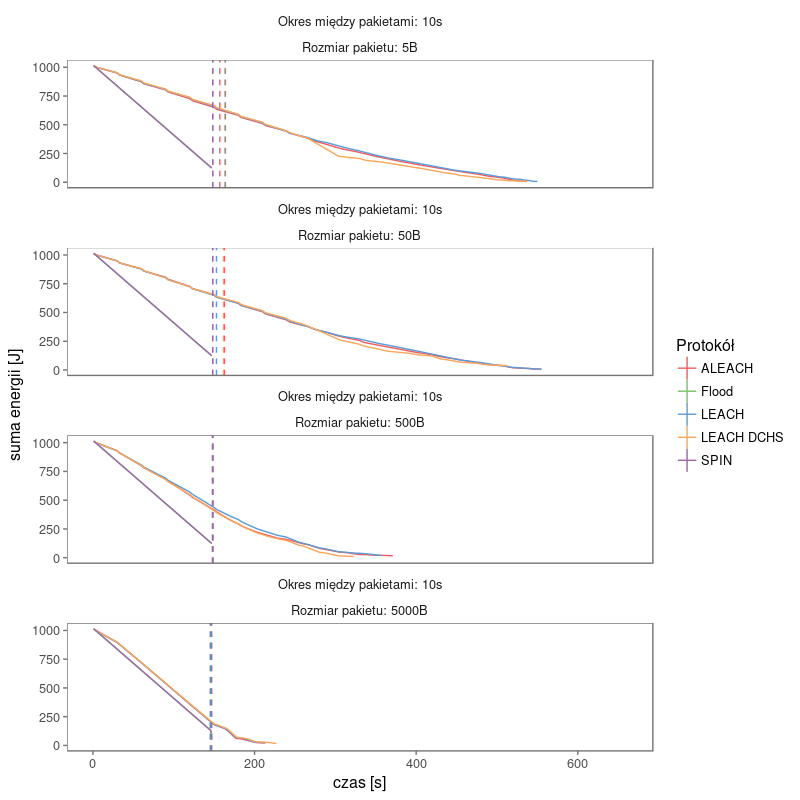
\includegraphics[scale=0.7]{\ImgPath/charts/stored_energy_normal_200sensors_col2.png}
	\end{center}
	\caption{Energia sieci - 200 czujników, rozkład normalny, okres pomiędzy pakietami: 10s}
\end{figure}

\begin{figure}[H]
	\begin{center}
		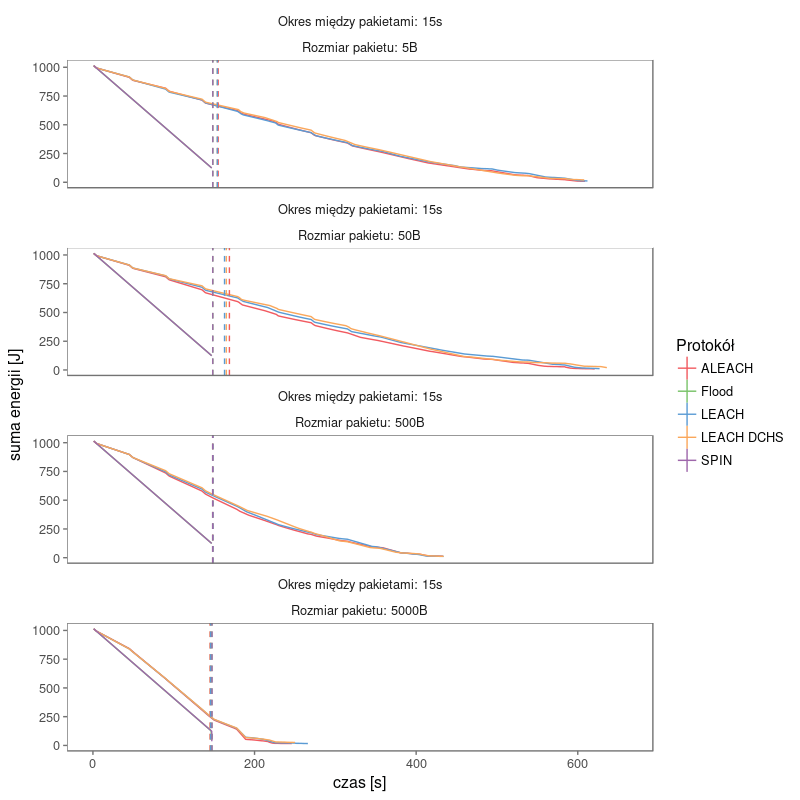
\includegraphics[scale=0.7]{\ImgPath/charts/stored_energy_normal_200sensors_col3.png}
	\end{center}
	\caption{Energia sieci - 200 czujników, rozkład normalny, okres pomiędzy pakietami: 15s}
\end{figure}

\begin{figure}[H]
	\begin{center}
		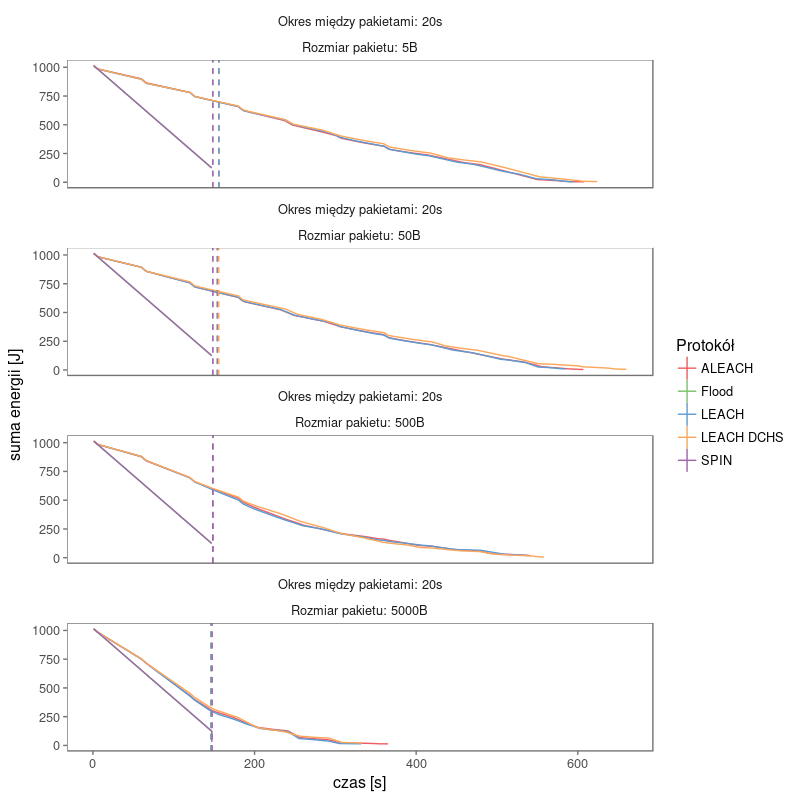
\includegraphics[scale=0.7]{\ImgPath/charts/stored_energy_normal_200sensors_col4.png}
	\end{center}
	\caption{Energia sieci - 200 czujników, rozkład normalny, okres pomiędzy pakietami: 20s}
\end{figure}

\begin{figure}[H]
	\begin{center}
		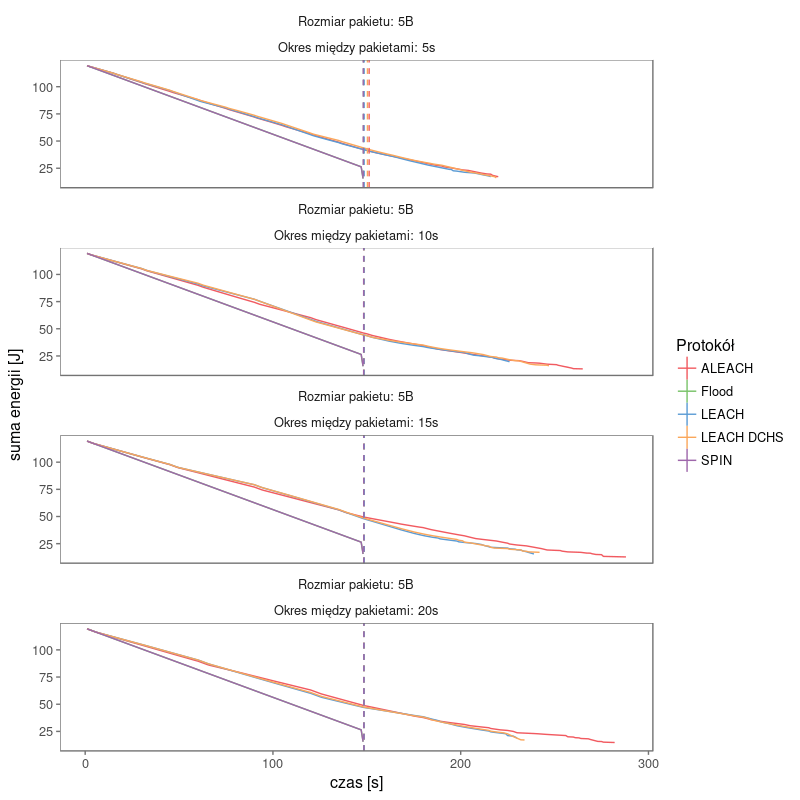
\includegraphics[scale=0.7]{\ImgPath/charts/stored_energy_uniform_20sensors_row1.png}
	\end{center}
	\caption{Energia sieci - 20 czujników, rozkład jednorodny, rozmiar pakietu: 5B}
\end{figure}

\begin{figure}[H]
	\begin{center}
		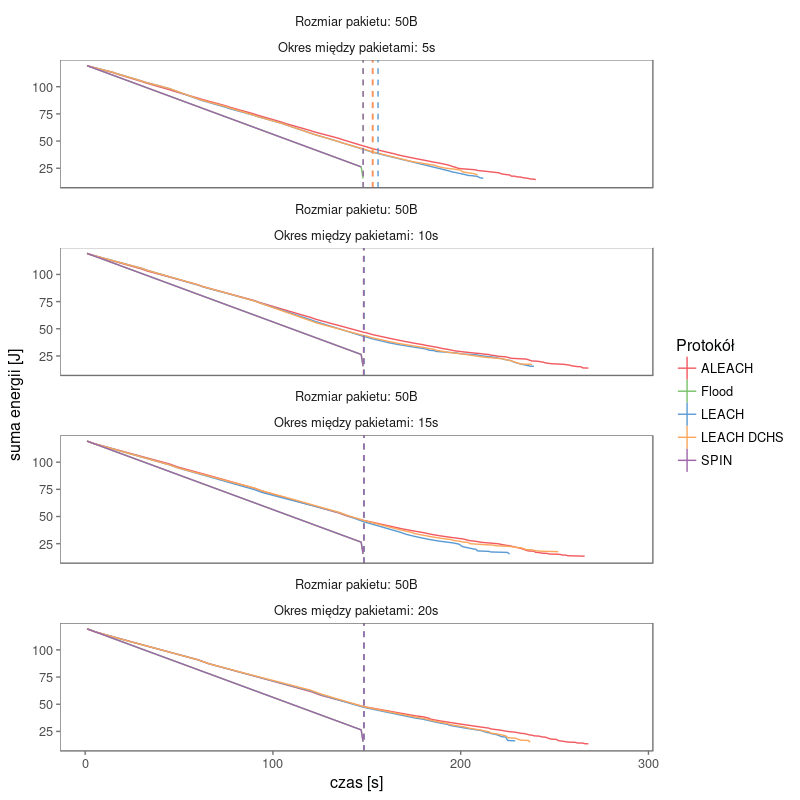
\includegraphics[scale=0.7]{\ImgPath/charts/stored_energy_uniform_20sensors_row2.png}
	\end{center}
	\caption{Energia sieci - 20 czujników, rozkład jednorodny, rozmiar pakietu: 50B}
\end{figure}

\begin{figure}[H]
	\begin{center}
		\includegraphics[scale=0.7]{\ImgPath/charts/stored_energy_uniform_20sensors_row3.png}
	\end{center}
	\caption{Energia sieci - 20 czujników, rozkład jednorodny, rozmiar pakietu: 500B}
\end{figure}

\begin{figure}[H]
	\begin{center}
		\includegraphics[scale=0.7]{\ImgPath/charts/stored_energy_uniform_20sensors_row4.png}
	\end{center}
	\caption{Energia sieci - 20 czujników, rozkład jednorodny, rozmiar pakietu: 5000B}
\end{figure}

\begin{figure}[H]
	\begin{center}
		\includegraphics[scale=0.7]{\ImgPath/charts/stored_energy_uniform_20sensors_col1.png}
	\end{center}
	\caption{Energia sieci - 20 czujników, rozkład jednorodny, okres pomiędzy pakietami: 5s}
\end{figure}

\begin{figure}[H]
	\begin{center}
		\includegraphics[scale=0.7]{\ImgPath/charts/stored_energy_uniform_20sensors_col2.png}
	\end{center}
	\caption{Energia sieci - 20 czujników, rozkład jednorodny, okres pomiędzy pakietami: 10s}
\end{figure}

\begin{figure}[H]
	\begin{center}
		\includegraphics[scale=0.7]{\ImgPath/charts/stored_energy_uniform_20sensors_col3.png}
	\end{center}
	\caption{Energia sieci - 20 czujników, rozkład jednorodny, okres pomiędzy pakietami: 15s}
\end{figure}

\begin{figure}[H]
	\begin{center}
		\includegraphics[scale=0.7]{\ImgPath/charts/stored_energy_uniform_20sensors_col4.png}
	\end{center}
	\caption{Energia sieci - 20 czujników, rozkład jednorodny, okres pomiędzy pakietami: 20s}
\end{figure}

\begin{figure}[H]
	\begin{center}
		\includegraphics[scale=0.7]{\ImgPath/charts/stored_energy_uniform_200sensors_row1.png}
	\end{center}
	\caption{Energia sieci - 200 czujników, rozkład jednorodny, rozmiar pakietu: 5B}
\end{figure}

\begin{figure}[H]
	\begin{center}
		\includegraphics[scale=0.7]{\ImgPath/charts/stored_energy_uniform_200sensors_row2.png}
	\end{center}
	\caption{Energia sieci - 200 czujników, rozkład jednorodny, rozmiar pakietu: 50B}
\end{figure}

\begin{figure}[H]
	\begin{center}
		\includegraphics[scale=0.7]{\ImgPath/charts/stored_energy_uniform_200sensors_row3.png}
	\end{center}
	\caption{Energia sieci - 200 czujników, rozkład jednorodny, rozmiar pakietu: 500B}
\end{figure}

\begin{figure}[H]
	\begin{center}
		\includegraphics[scale=0.7]{\ImgPath/charts/stored_energy_uniform_200sensors_row4.png}
	\end{center}
	\caption{Energia sieci - 200 czujników, rozkład jednorodny, rozmiar pakietu: 5000B}
\end{figure}

\begin{figure}[H]
	\begin{center}
		\includegraphics[scale=0.7]{\ImgPath/charts/stored_energy_uniform_200sensors_col1.png}
	\end{center}
	\caption{Energia sieci - 200 czujników, rozkład jednorodny, okres pomiędzy pakietami: 5s}
\end{figure}

\begin{figure}[H]
	\begin{center}
		\includegraphics[scale=0.7]{\ImgPath/charts/stored_energy_uniform_200sensors_col2.png}
	\end{center}
	\caption{Energia sieci - 200 czujników, rozkład jednorodny, okres pomiędzy pakietami: 10s}
\end{figure}

\begin{figure}[H]
	\begin{center}
		\includegraphics[scale=0.7]{\ImgPath/charts/stored_energy_uniform_200sensors_col3.png}
	\end{center}
	\caption{Energia sieci - 200 czujników, rozkład jednorodny, okres pomiędzy pakietami: 15s}
\end{figure}

\begin{figure}[H]
	\begin{center}
		\includegraphics[scale=0.7]{\ImgPath/charts/stored_energy_uniform_200sensors_col4.png}
	\end{center}
	\caption{Energia sieci - 200 czujników, rozkład jednorodny, okres pomiędzy pakietami: 20s}
\end{figure}

\end{document}